\documentclass[11pt,letterpaper]{article}

% Main document
% !TEX root = main.tex
\usepackage[margin=1in]{geometry}
\usepackage{amsmath}
\usepackage{amssymb}
\usepackage{graphicx}
\usepackage{hyperref}
\usepackage[backend=biber,style=numeric]{biblatex}
\addbibresource{bibliography.bib}
\title{From Electronic Structure to Continuum Response:A Computational Model for Strain-Dependent Conductivity in Piezoresistive Materials}
\author{Shah Yusuf Safi}
\date{\today}

%\usepackage{amsthm}
%
%
%
%% theorem like envs
%
%\theoremstyle{defination}
%
%%\newtheorem{envname}{caption}[within]
%
%\newtheorem{defination}{Defination}[section]


% engineering style definitions

\usepackage{mdframed}
\usepackage{xcolor}
\usepackage{tabularx} 
\usepackage{booktabs}
\usepackage{siunitx} % style
%\usepackage[draft]{graphicx} % draft mode


\newmdtheoremenv[
  linewidth=0.5pt,
  linecolor=black,
  backgroundcolor=gray!5,
]{definition}{Definition}[section]


\newmdtheoremenv[
  linewidth=0.3pt,
  linecolor=blue,
  backgroundcolor=blue!5,
]{example}{Example}[section]


\newmdtheoremenv[
  linewidth=0.3pt,
  linecolor=blue,
  backgroundcolor=purple!5,
]{proposition}{Proposition}[section]



\newmdtheoremenv[
  linewidth=0.3pt,
  linecolor=blue,
  backgroundcolor=black!5,
]{theorem}{Theorem}[section]




\newmdtheoremenv[
  linewidth=0.1pt,
  linecolor=blue,
  backgroundcolor=green!9,
]{proof}{Proof}[section]


\newmdtheoremenv[
  linewidth=0.1pt,
  linecolor=blue,
  backgroundcolor=green!5,
]{remark}{Remark}[section]

\newmdtheoremenv[
  linewidth=0.1pt,
  linecolor=red,
]{RL}{Review Later}

% Basic graphics
\usepackage{graphicx}

% Optional figures without errors
\usepackage{ifthen}

% Simple verbatim code blocks
% Simple verbatim code blocks
\usepackage{fancyvrb}
\DefineVerbatimEnvironment{codeblock}{Verbatim}{fontsize=\small,frame=single}



\newcommand{\Var}{\operatorname{Var}}
\DeclareMathOperator{\Cov}{Cov}






\begin{document}
\maketitle

\begin{abstract}

Many sensing devices rely on transduction mechanisms that convert mechanical deformation into measurable electrical signals.
A prominent example is the piezoresistive effect, where the electrical conductivity of a material varies under applied strain.

From a materials physics perspective, this behavior originates from strain-induced modifications of the electronic structure and carrier transport properties. 
Mechanical deformation alters band energies, effective masses, and scattering mechanisms, which in turn influence carrier mobility and electrical conductivity \cite{hamaguchi}. 
In certain regimes, additional effects such as tunneling may also contribute to the overall response.

This work develops a computational framework for modeling strain-dependent conductivity in deformable materials by connecting these physical mechanisms across scales.
At the continuum level, the mechanical behavior is described by the equations of elasticity, while the electrical response is governed by a conductivity equation with strain-dependent coefficients. 
This leads to a coupled system of partial differential equations of the form
\[
\nabla \cdot \boldsymbol{\sigma}(u) = 0, \qquad
\nabla \cdot \left( \sigma(\varepsilon(u)) \nabla V \right) = 0,
\]
where $u$ denotes the displacement field, $V$ the electrical potential, and $\sigma(\varepsilon(u))$ represents an effective conductivity incorporating the influence of mechanical deformation.

A central aspect of this study is the interpretation of the constitutive relation $\sigma(\varepsilon)$.
Rather than treating it purely phenomenologically, the framework is designed so that it can be informed by transport models derived from electronic structure calculations, providing a physically motivated link between microscopic behavior and macroscopic response.

From a computational perspective, the focus lies on the formulation and numerical solution of the coupled system using finite element methods.
A baseline case with constant conductivity is first analyzed and validated, followed by the extension to spatially varying, strain-dependent conductivity.
The framework is constructed to remain flexible, allowing the incorporation of physics-based models or data-driven approximations for $\sigma(\varepsilon)$.

The proposed approach provides a consistent and extensible pathway for studying electromechanical coupling in materials.
Potential applications include sensing technologies, flexible electronics, and structural health monitoring.

\end{abstract}

\tableofcontents

% Sections
% ================================
% INTRODUCTION
% ================================
\section{Introduction}
\label{sec:introduction}

The piezoresistive effect arises from the coupling between mechanical deformation 
and electrical conduction. In typical applications, a doped semiconductor element 
(such as silicon) is embedded within a mechanical structure, where external forces 
induce strain in the material. This deformation alters the electronic transport properties 
of the material, leading to measurable changes in its electrical response, commonly observed 
as variations in voltage or resistance.

\begin{figure}[htbp]
    \centering
    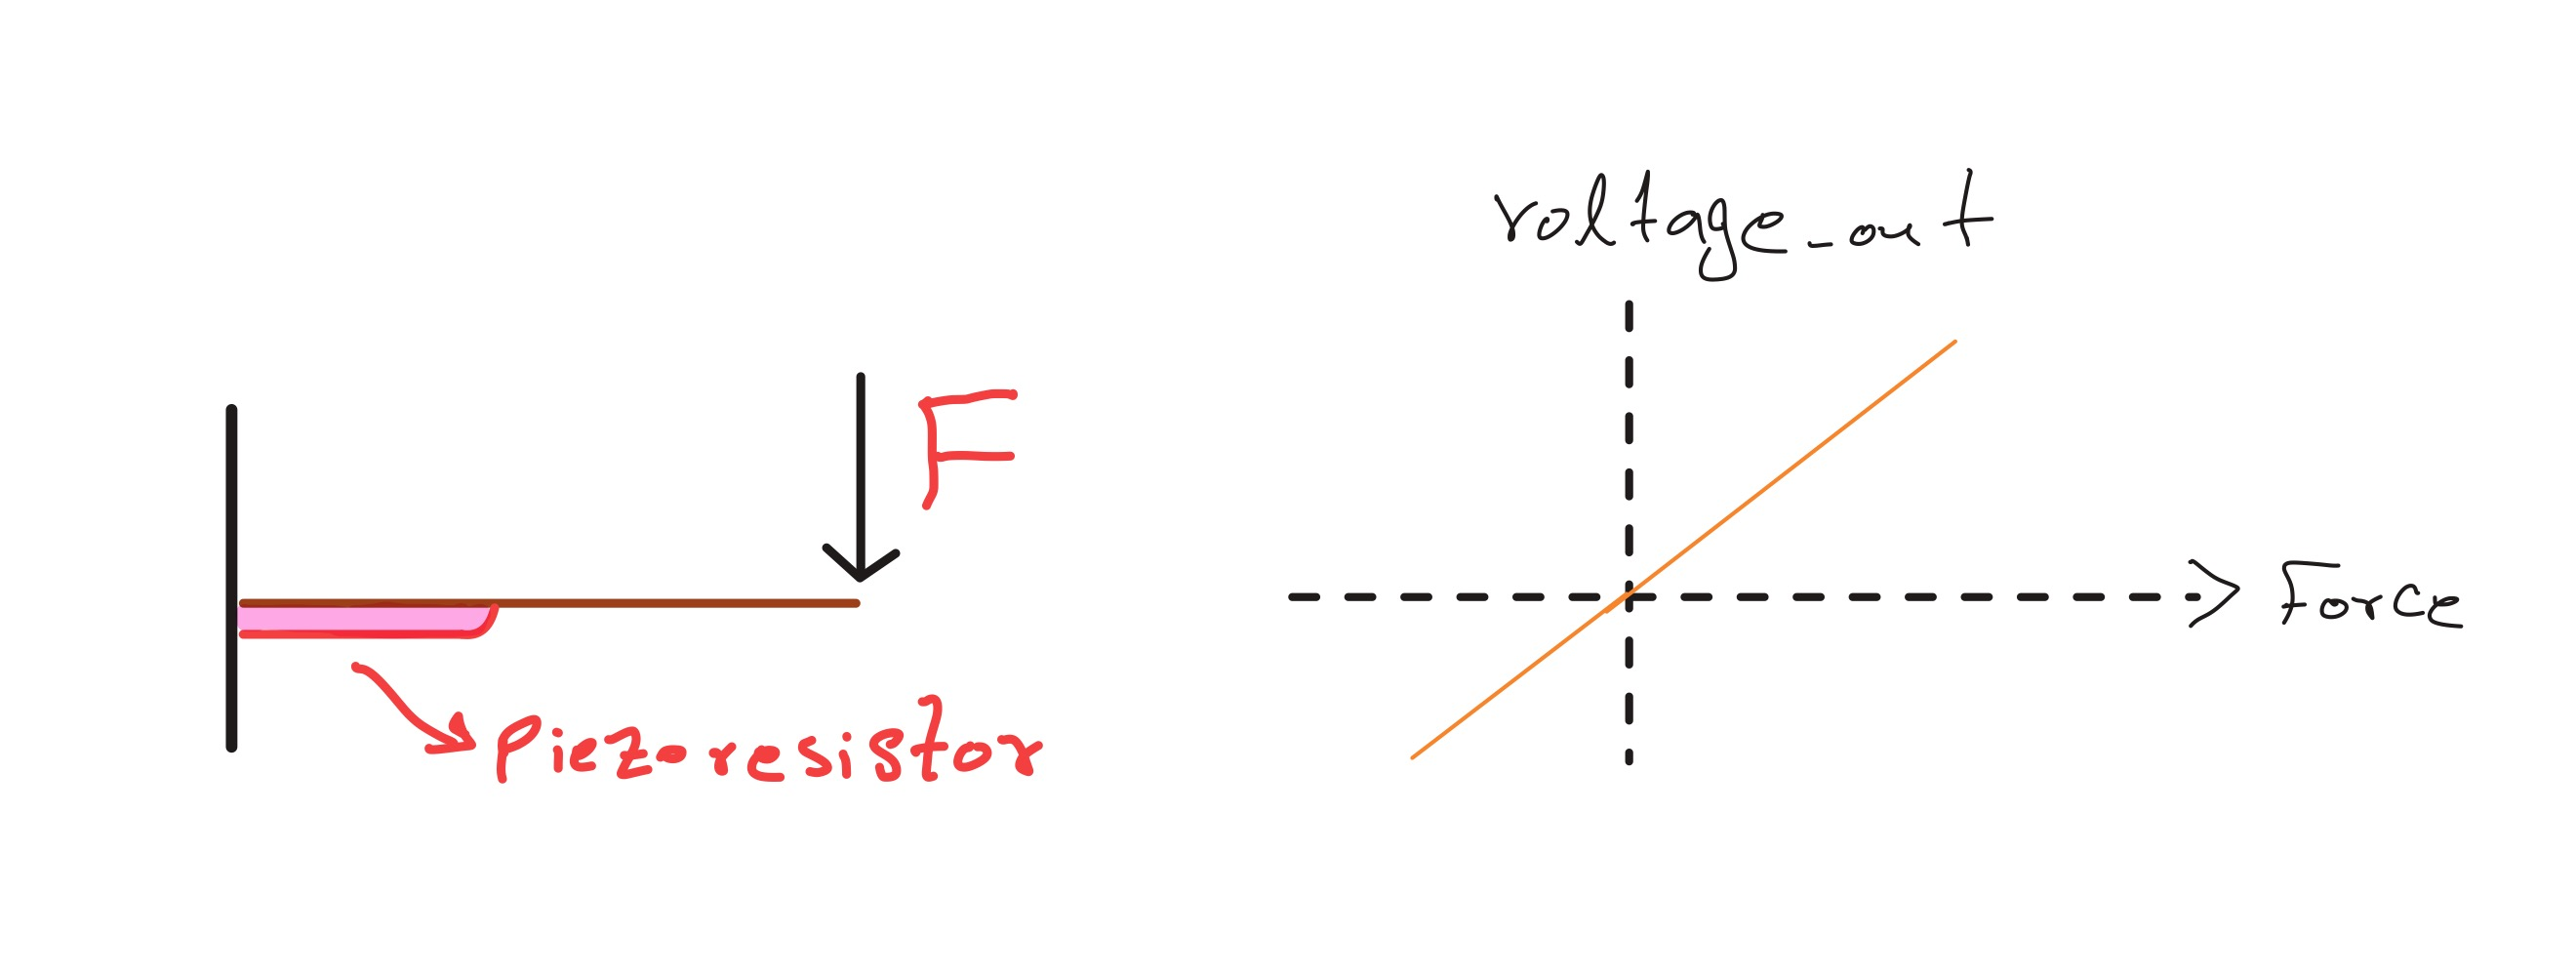
\includegraphics[width=0.5\textwidth]{Images/phenomenon.jpeg}
    \caption{A schematic representation of the piezoresistive effect, where mechanical deformation leads to changes in electrical response.}
\end{figure}

The piezoresistive effect, first observed by William Thomson (Lord Kelvin) 
in the 19th century and later developed for semiconductors by Bardeen, Shockley, and Smith \cite{smith1954}, 
describes the dependence of electrical conductivity on mechanical deformation. 
At a microscopic level, this behavior originates from strain-induced modifications of the electronic structure 
and carrier transport mechanisms. In particular, quantities such as band energies, effective masses, and 
scattering processes are affected by deformation, which in turn influence carrier mobility and conductivity \cite{hamaguchi}.

There exists a wide spectrum of engineering realizations of the piezoresistive effect, 
including strain gauges, pressure sensors, microelectromechanical systems (MEMS), 
cantilever-based sensing devices, and flexible or wearable systems \cite{doll2013}. 
Although these systems differ in geometry, material composition, and boundary conditions, 
they can be interpreted as different realizations of the same underlying electromechanical coupling.

Despite extensive technological development and optimization, the modeling of this coupling 
is often carried out in a phenomenological and application-specific manner, where the dependence 
of conductivity on strain is introduced empirically. From a computational materials perspective, 
this raises a more fundamental question: how can such macroscopic descriptions be related in a 
consistent way to the underlying physical mechanisms governing electronic transport?

The present work approaches this problem by developing a computational framework in which 
the electromechanical coupling is described at the continuum level, while maintaining a clear 
connection to the underlying transport physics. In this setting, the continuum model serves as 
an effective description of strain-dependent conductivity, acting as a bridge between microscopic 
electronic behavior and macroscopic response.





\section{Phenomena of piezoresistivity}
\label{sec:piezoresistivity}



\section{Continum Model Formulation}
\label{sec:ContinumModel}


\section{Numerical Solution of the continumm problem}
\label{sec:FEM}



\section{Essentials of Strain and Stress Analysis}
\label{sec:StrainStress}



\section{Symmetry and operations analysis of the crystaline Si}
\label{sec:Symmetry}

\section{Deformation Potentials}
\label{sec:DPT}

\section{Results and discussions}
\label{sec:results}


\section{Error analysis}
\label{sec:Error}


% ================================
% PROBLEM ARTICULATION
% ================================
\section{Problem Articulation}

At the continuum level, electrical conduction in a deformable material can be described 
by a conductivity equation in which the electrical conductivity depends on the local mechanical strain. 
Such models are widely used in engineering applications and can be solved efficiently using numerical methods. 
However, the central quantity in this description, namely the strain-dependent conductivity $\sigma(\varepsilon)$, 
is often introduced phenomenologically, without an explicit connection to the underlying material physics.

From a materials physics perspective, this raises a fundamental question: 
how does mechanical deformation at the atomic scale translate into a change in macroscopic electrical conductivity?

In semiconductors, strain modifies the crystal structure and therefore the electronic band structure of the material. 
This leads to changes in quantities such as band energies, effective masses, and carrier velocities. 
As a consequence, the transport properties of charge carriers are altered, affecting mobility and electrical conductivity. 
These mechanisms are described in semiconductor theory through band-structure analysis and transport models 
such as the semiclassical Boltzmann transport equation \cite{hamaguchi}.

This observation suggests a natural multiscale structure of the problem. 
At the microscopic level, strain influences the electronic structure of the material. 
At the transport level, the modified electronic structure determines carrier dynamics and effective conductivity. 
At the continuum level, this conductivity enters as a constitutive parameter in the electrical conduction equation.

From a transport perspective, the electrical conductivity can be expressed using the semiclassical Boltzmann transport equation as

\begin{equation}
\sigma_{ij} = \frac{e^2}{4\pi^3}\sum_n \int v_i^n(\mathbf{k})\, v_j^n(\mathbf{k})\, \tau_n(\mathbf{k})
\left(-\frac{\partial f_0}{\partial E}\right) d\mathbf{k},
\end{equation}

where $v_i^n(\mathbf{k})$ denotes the group velocity of electrons in band $n$, $\tau_n$ is the relaxation time, 
and $f_0$ is the equilibrium distribution function.

Mechanical deformation enters this description through strain-induced shifts in the electronic band structure, 
which can be modeled using deformation potential theory,

\begin{equation}
\delta E_n = \Xi_{ij}\,\varepsilon_{ij},
\end{equation}

where $\Xi_{ij}$ denotes the deformation potential tensor.

Together, these relations provide a microscopic interpretation of the strain-dependent conductivity $\sigma(\varepsilon)$ 
used in the continuum model.

The core challenge of this work is therefore to connect these levels in a computationally consistent way. 
Rather than treating $\sigma(\varepsilon)$ purely as a fitting function, the goal is to interpret it as an effective quantity 
that reflects underlying electronic and transport mechanisms, while remaining suitable for use in continuum simulations.

This perspective allows the continuum model to serve not only as a numerical tool, but also as a bridge between 
microscopic physical processes and macroscopic device behavior.

The multiscale structure of the problem can be summarized as follows:

\begin{center}
\begin{tabular}{lll}
\textbf{Scale} & \textbf{Description} & \textbf{Typical Tool} \\
\hline
Electronic & Band structure $E_n(\mathbf{k}, \varepsilon)$ & DFT  \\
Transport  & Conductivity $\sigma(\varepsilon)$ & Boltzmann transport \\
Continuum  & Fields $V, \mathbf{E}, \mathbf{J}$ & FEM \\
\end{tabular}
\end{center}

In particular, this framework enables the incorporation of physically informed or data-driven constitutive relations, depending on the level of detail available for the underlying material.

\section{Problem Statement and Motivation}

Consider a conductive element with length $L$, cross-sectional area $A$, and resistivity $\rho$. 
Its electrical resistance is given by

\begin{equation}
    R = \frac{\rho L}{A}.
\end{equation}

Under mechanical loading, both the geometry and the intrinsic material properties of the conductor may change. 
In particular, the length, cross-sectional area, and resistivity become functions of deformation, 
making the resistance dependent on the mechanical state.

Using Ohm's law,

\begin{equation}
    R = \frac{V}{I},
\end{equation}

and expressing voltage and current in terms of field quantities,

\begin{equation}
    V = EL, \qquad I = JA,
\end{equation}

we obtain

\begin{equation}
    \frac{EL}{JA} = \frac{\rho L}{A}.
\end{equation}

Canceling the geometric factors $L$ and $A$ leads to the local relation

\begin{equation}
    \mathbf{J} = \sigma \mathbf{E}, \qquad \sigma = \frac{1}{\rho},
\end{equation}

where $\mathbf{E} = -\nabla V$ is the electric field. 
This formulation expresses Ohm’s law in a local (continuum) form, independent of the specific geometry 
and applicable to spatially varying fields.

Combining this with charge conservation in the steady state,

\begin{equation}
    \nabla \cdot \mathbf{J} = 0,
\end{equation}

yields the conductivity equation

\begin{equation}
    \nabla \cdot (\sigma \nabla V) = 0.
\end{equation}

This equation provides a continuum description of electrical conduction in materials, 
where the conductivity $\sigma$ may vary spatially. It belongs to the class of elliptic partial differential equations 
in divergence form \cite{evans}.

In piezoresistive materials, the key feature is that the conductivity is no longer constant, but depends on the mechanical deformation of the material. 
At a macroscopic level, this dependence can be expressed as

\begin{equation}
    \sigma = \sigma(\varepsilon(u)),
\end{equation}

where the strain tensor is given by\footnote{The strain tensor is defined as the symmetric part of the displacement gradient, which removes rigid body rotations and captures the true deformation of the material.}

\begin{equation}
    \varepsilon(u) = \frac{1}{2}(\nabla u + \nabla u^T).
\end{equation}

This relation can be interpreted as an effective description of how mechanical deformation influences electrical transport. 
From a physical perspective, the dependence of conductivity on strain originates from strain-induced modifications of the electronic structure 
and carrier transport properties, which are affected by lattice deformation \cite{hamaguchi}.

The resulting model therefore introduces a nonlinear coupling between mechanical deformation and electrical conduction: 
the mechanical field $u$ determines the strain $\varepsilon(u)$, which modifies the conductivity $\sigma$, and this in turn affects 
the electrical potential $V$ through the conductivity equation.

\begin{figure}[htbp]
    \centering
    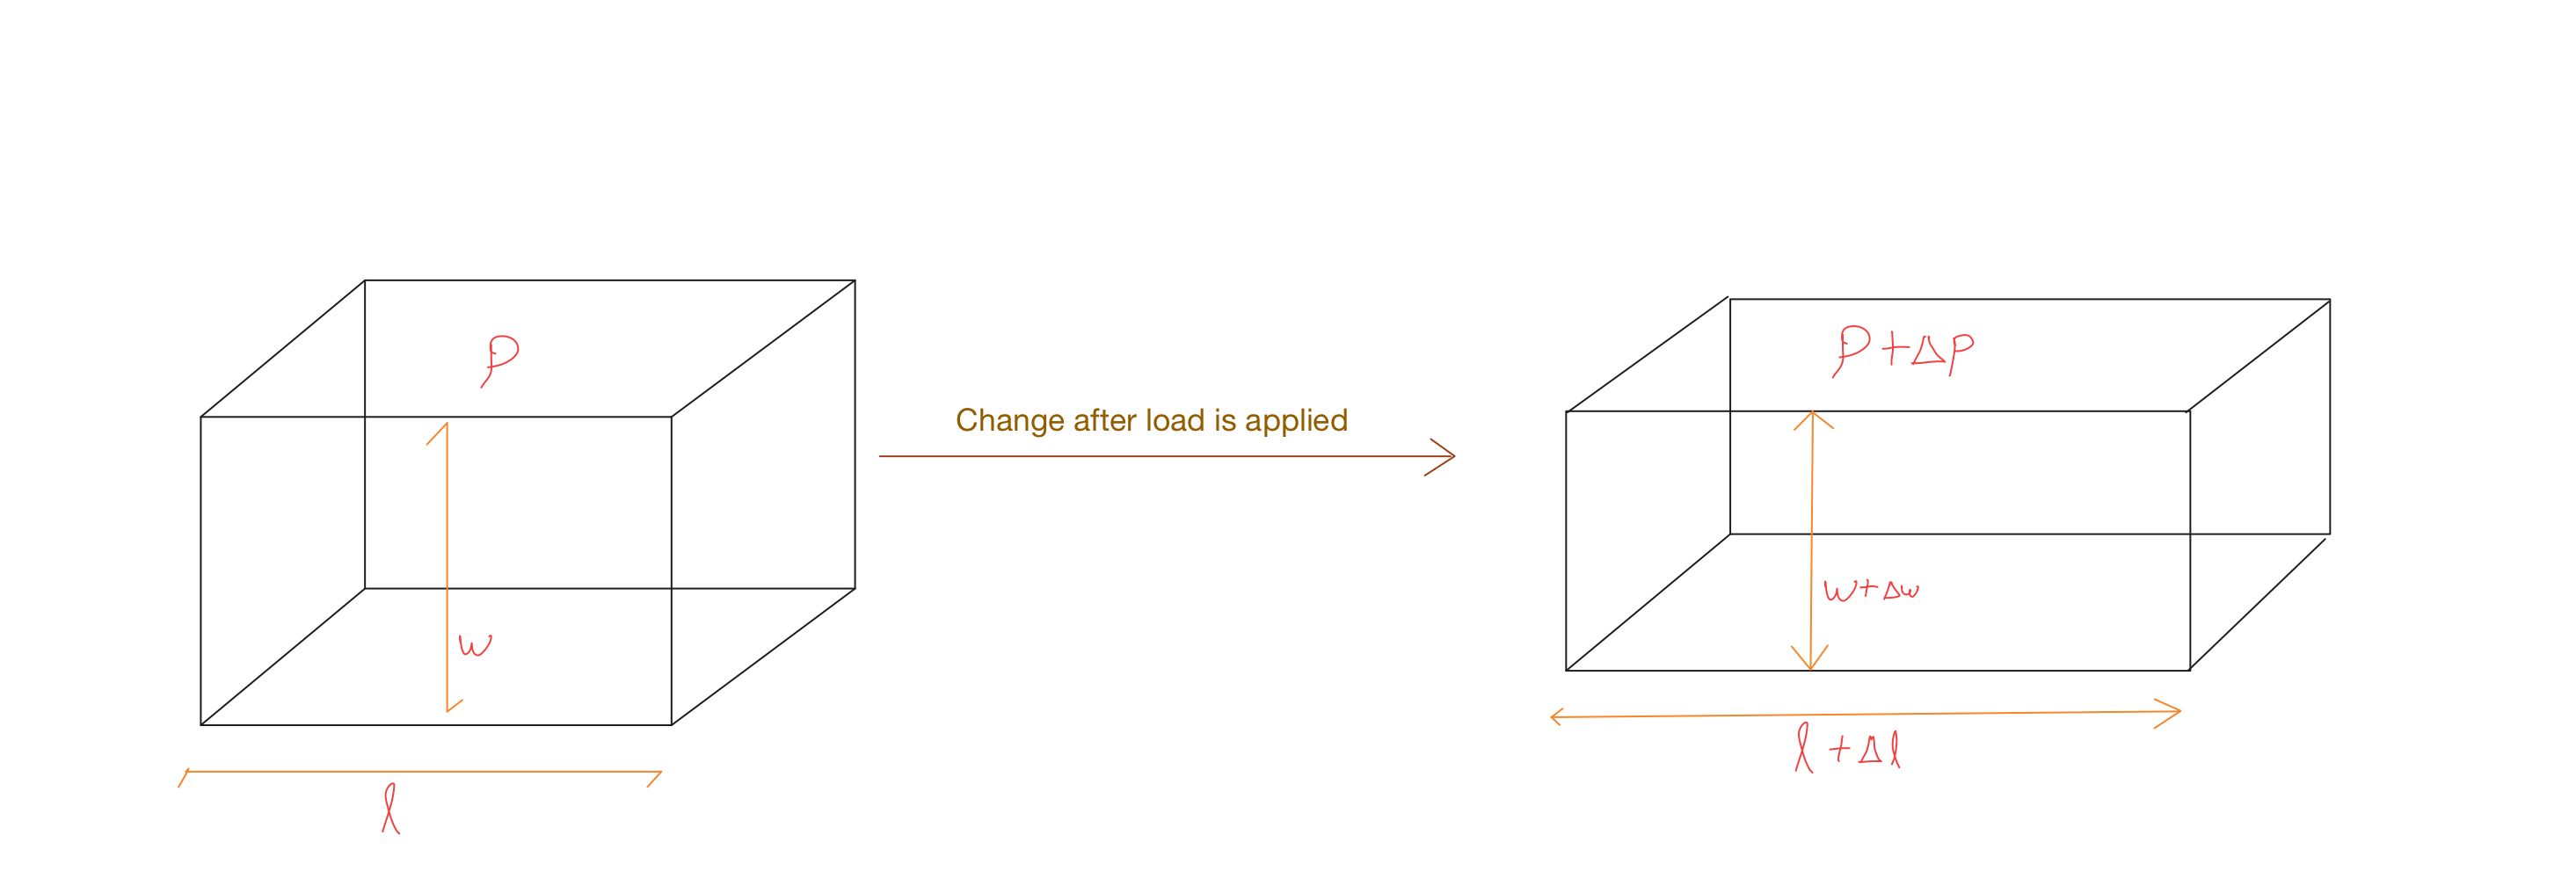
\includegraphics[width=0.7\textwidth]{Images/model1.png}
    \caption{Change of geometric and material properties under mechanical deformation. 
    $L$ denotes the length of the conductor, $W$ its characteristic width, and $A = W^2$ the cross-sectional area (assuming a square cross-section). 
    The material property $\rho$ represents the electrical resistivity, which may vary under mechanical deformation. 
    Both geometric changes and intrinsic material variations contribute to the overall change in resistance.}
\end{figure}

This illustrates that both geometric deformation and intrinsic material changes contribute to the variation of resistance, 
providing the basis for modeling the piezoresistive effect within a continuum framework.

\section{Mathematical Model}
\label{sec:math model}

Based on the physical considerations discussed above, the electromechanical behavior 
of the material is described at the continuum level by a coupled system of partial differential equations.

The mechanical response is governed by the equations of elasticity,

\begin{equation}
    \label{eq:conductivity}
    \nabla \cdot \boldsymbol{\sigma}(u) = 0,
\end{equation}

where $u$ denotes the displacement field and $\boldsymbol{\sigma}(u)$ is the stress tensor, 
which depends on the strain through a constitutive relation.

The electrical response is described by the conductivity equation,

\begin{equation}
    \label{eq:1d-cond}
    \nabla \cdot \left( \sigma(\varepsilon(u)) \nabla V \right) = 0,
\end{equation}

where $V$ is the electrical potential and the conductivity $\sigma$ depends on the strain tensor 
$\varepsilon(u)$.

Together, these equations define a coupled system in which the mechanical field $u$ determines 
the strain $\varepsilon(u)$, which in turn modifies the conductivity $\sigma$, and thereby 
influences the electrical potential $V$.

From a physical perspective, this coupling provides an effective continuum description of how 
mechanical deformation alters the underlying electronic transport properties of the material.

The system is nonlinear due to the dependence of the conductivity on the strain field.

This formulation serves as the basis for the computational modeling of the piezoresistive effect, 
linking continuum mechanics with strain-dependent electrical conduction.



\section{State of Research}

The piezoresistive effect has been extensively investigated in both experimental and engineering contexts, 
particularly in semiconductor-based sensors and microelectromechanical systems (MEMS) \cite{smith1954,doll2013}. 
Early studies established the strong dependence of electrical conductivity on mechanical strain in materials such as silicon, 
highlighting the importance of crystal structure and carrier transport in determining the sensitivity of the effect.

From a materials physics perspective, piezoresistivity originates from strain-induced modifications of the electronic structure 
and charge transport properties. Mechanical deformation can alter band structure, effective masses, and scattering mechanisms, 
which in turn influence carrier mobility and electrical conductivity \cite{hamaguchi}. 
These effects are well understood at the microscopic and transport levels.

In practical modeling and engineering applications, however, this coupling is typically introduced in a simplified manner, 
where the conductivity is treated as an empirical function of strain. While such approaches are effective for device design, 
they do not provide a transparent link between microscopic transport mechanisms and macroscopic behavior.

At the continuum level, partial differential equation models are widely used to describe both elasticity and electrical conduction. 
Nevertheless, the incorporation of strain-dependent transport properties into these models is usually carried out phenomenologically, 
without a systematic connection to the underlying physics.

This reveals a gap between physically grounded transport descriptions and continuum-level modeling. 
Bridging this gap in a computationally consistent way remains an open and relevant problem, particularly for materials and devices 
where electromechanical coupling plays a central role.

Based on these considerations, the proposed study is guided by the following research questions:

\begin{itemize}
    \item How can strain-dependent conductivity be incorporated into a consistent continuum model of electromechanical coupling?
    \item How does mechanical deformation influence the spatial distribution of electrical potential in conductive materials?
    \item What effects arise from the nonlinear coupling between mechanics and electrical transport?
    \item To what extent can flexible (e.g.\ data-driven or physics-informed) approaches improve the modeling of $\sigma(\varepsilon)$?
\end{itemize}

To address these questions, the study is structured around the following components:

\begin{itemize}
    \item Physical background and modeling assumptions
    \item Formulation of the coupled electromechanical model
    \item Analysis of the nonlinear system
    \item Computational methods and numerical experiments
    \item Interpretation of results in the context of material behavior
\end{itemize}

\section{Methodology}

The proposed study follows a computational approach based on a continuum description of the coupled electromechanical system. 
The methodology is structured in several stages, combining physical modeling with numerical approximation.

First, the governing equations of elasticity and electrical conduction are formulated within a consistent continuum framework. 
The mechanical problem provides the displacement field $u$, from which the strain tensor $\varepsilon(u)$ is computed. 
This strain field enters the electrical problem through the strain-dependent conductivity $\sigma(\varepsilon)$.

As a baseline, the electrical conduction problem with constant conductivity is considered and solved numerically. 
This case admits an analytical solution and serves to validate the numerical implementation. 
A finite element discretization is employed, and the numerical solution is compared against the exact solution to ensure correctness.

\begin{figure}[htbp]
    \centering
    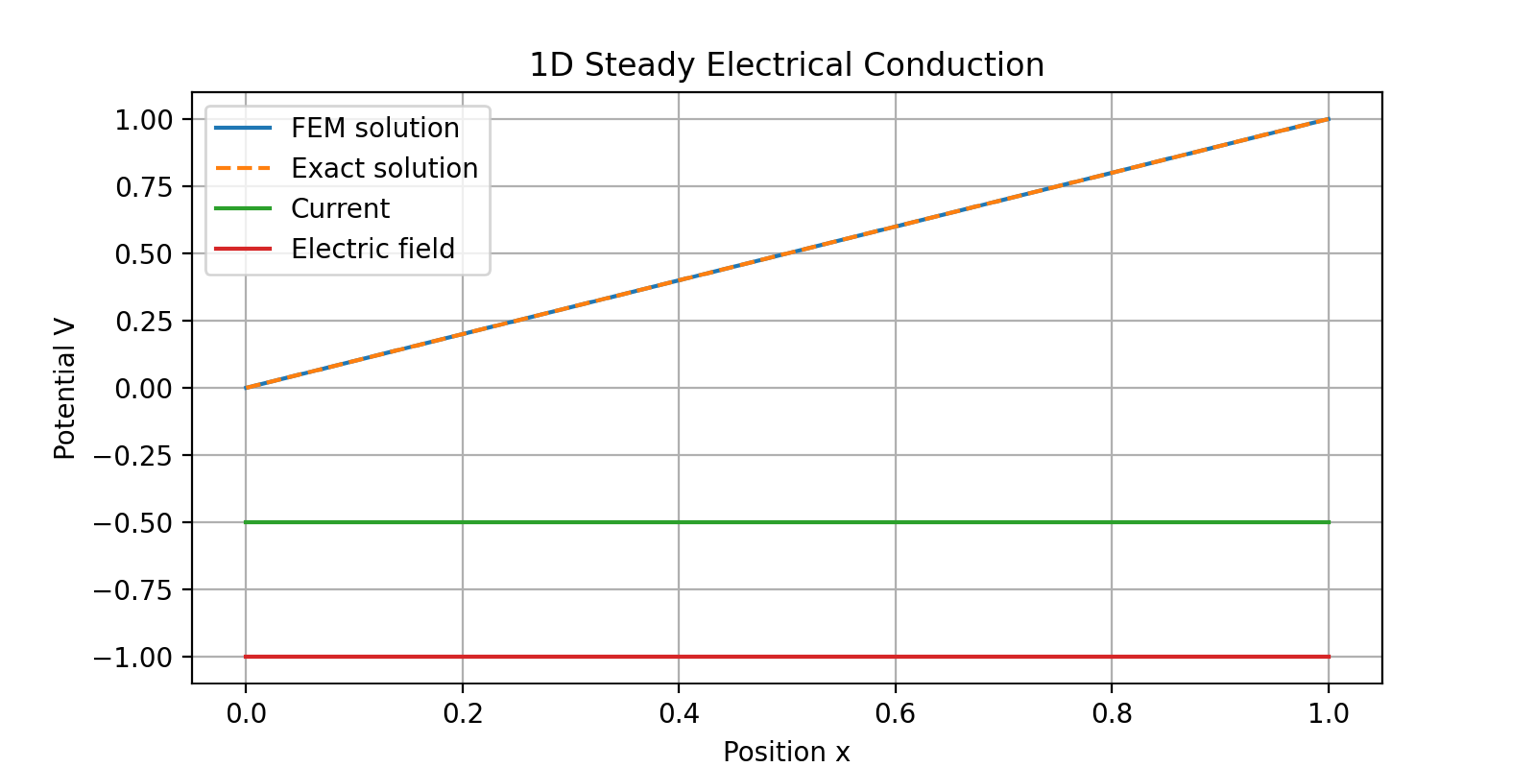
\includegraphics[width=0.75\textwidth]{Images/1d_cond.png}
    \caption{Finite element solution of the 1D steady conduction problem with constant conductivity compared with the analytical solution. 
    The linear potential profile and constant electric field confirm the expected physical behavior.}
\end{figure}

This baseline case also provides a reference for interpreting deviations introduced by strain-dependent conductivity in the coupled problem.

Building on this, the full coupled system is addressed by introducing a spatially varying conductivity $\sigma(\varepsilon(u))$. 
The problem is solved iteratively: starting from an initial displacement field, the strain is computed, the conductivity is updated, 
and the electrical problem is solved. This procedure is repeated until convergence is achieved.

The resulting system is nonlinear due to the dependence of $\sigma$ on $\varepsilon(u)$, and particular attention is given to the stability 
and convergence of the numerical scheme, as well as to the sensitivity of the solution with respect to deformation.

From a computational perspective, the finite element method (FEM) is used as the primary discretization technique due to its flexibility 
in handling heterogeneous material properties and complex geometries. The implementation emphasizes clarity and modularity, allowing 
systematic exploration of different forms of the strain–conductivity relation.

Beyond purely phenomenological models, the framework is designed to accommodate physically motivated constitutive relations. 
In particular, the function $\sigma(\varepsilon)$ can be informed by transport models derived from electronic structure calculations, 
or approximated using data-driven approaches when such data is available.

Overall, the methodology provides a transparent and extensible computational pipeline that connects continuum modeling 
with physically grounded descriptions of strain-dependent conductivity.

\section{Parametric Solution}
\label{sec:parametric}

In modeling electromechanical transport, it is important to distinguish between
\emph{geometric effects} and \emph{material effects}. Geometric changes arise from
deformation of the domain (e.g., changes in length $L$ or cross-sectional area $A$),
which influence quantities such as resistance through the relation
\begin{equation}
    R = \frac{L}{A\,\sigma}.
    \label{eq:resistance}
\end{equation}
Material effects, in contrast, describe how intrinsic properties, such as the
electrical conductivity $\sigma$, change due to deformation. In semiconductors,
this latter effect---known as \emph{piezoresistivity}---is typically dominant
and is the focus of the present work.

To incorporate this dependence, the conductivity is treated as a function of the
mechanical strain,
\begin{equation}
    \sigma = \sigma(\varepsilon),
    \label{eq:sigma_eps}
\end{equation}
where $\varepsilon$ denotes a scalar strain measure derived from the strain tensor
$\varepsilon(\mathbf{u})$ introduced in Section~\ref{sec:math model}.\footnote{In the
one-dimensional setting considered here, $\varepsilon$ reduces to the axial
component $\varepsilon_{xx}$; the generalization to tensorial strain is
straightforward through the appropriate invariants.} The exact functional form of
$\sigma(\varepsilon)$ is generally unknown or analytically intractable when
derived from first-principles microscopic transport theory. For sufficiently
small deformations, however, $\sigma(\varepsilon)$ may be assumed smooth and
approximated by its Taylor expansion about the undeformed reference state
$\varepsilon = 0$:
\begin{equation}
    \sigma(\varepsilon)
    \approx \sigma_0
    + \left.\frac{d\sigma}{d\varepsilon}\right|_{0}\!\varepsilon
    + \frac{1}{2}\left.\frac{d^2\sigma}{d\varepsilon^2}\right|_{0}\!\varepsilon^{2}
    + \mathcal{O}(\varepsilon^{3}),
    \label{eq:taylor_raw}
\end{equation}
where $\sigma_0 = \sigma(0)$ is the reference (unstrained) conductivity.

Factoring out $\sigma_0$ yields the normalized form
\begin{equation}
    \sigma(\varepsilon)
    = \sigma_0\left(1 + \pi\,\varepsilon + \alpha\,\varepsilon^{2} + \dots\right),
    \label{eq:taylor_normalized}
\end{equation}
with the dimensionless coefficients
\begin{equation}
    \pi = \frac{1}{\sigma_0}\left.\frac{d\sigma}{d\varepsilon}\right|_{0},
    \qquad
    \alpha = \frac{1}{2\,\sigma_0}\left.\frac{d^2\sigma}{d\varepsilon^{2}}\right|_{0}.
    \label{eq:coeff_def}
\end{equation}
Here $\pi$ is the \emph{linear piezoresistive coefficient}, characterizing the
first-order sensitivity of the conductivity to strain, while $\alpha$ captures
higher-order nonlinear effects relevant at larger strain amplitudes. The
expansion~\eqref{eq:taylor_normalized} is not geometric in nature; rather, it
provides a local approximation of how the \emph{internal electronic transport
properties} of the material respond to deformation.

\begin{figure}[ht]
    \centering
    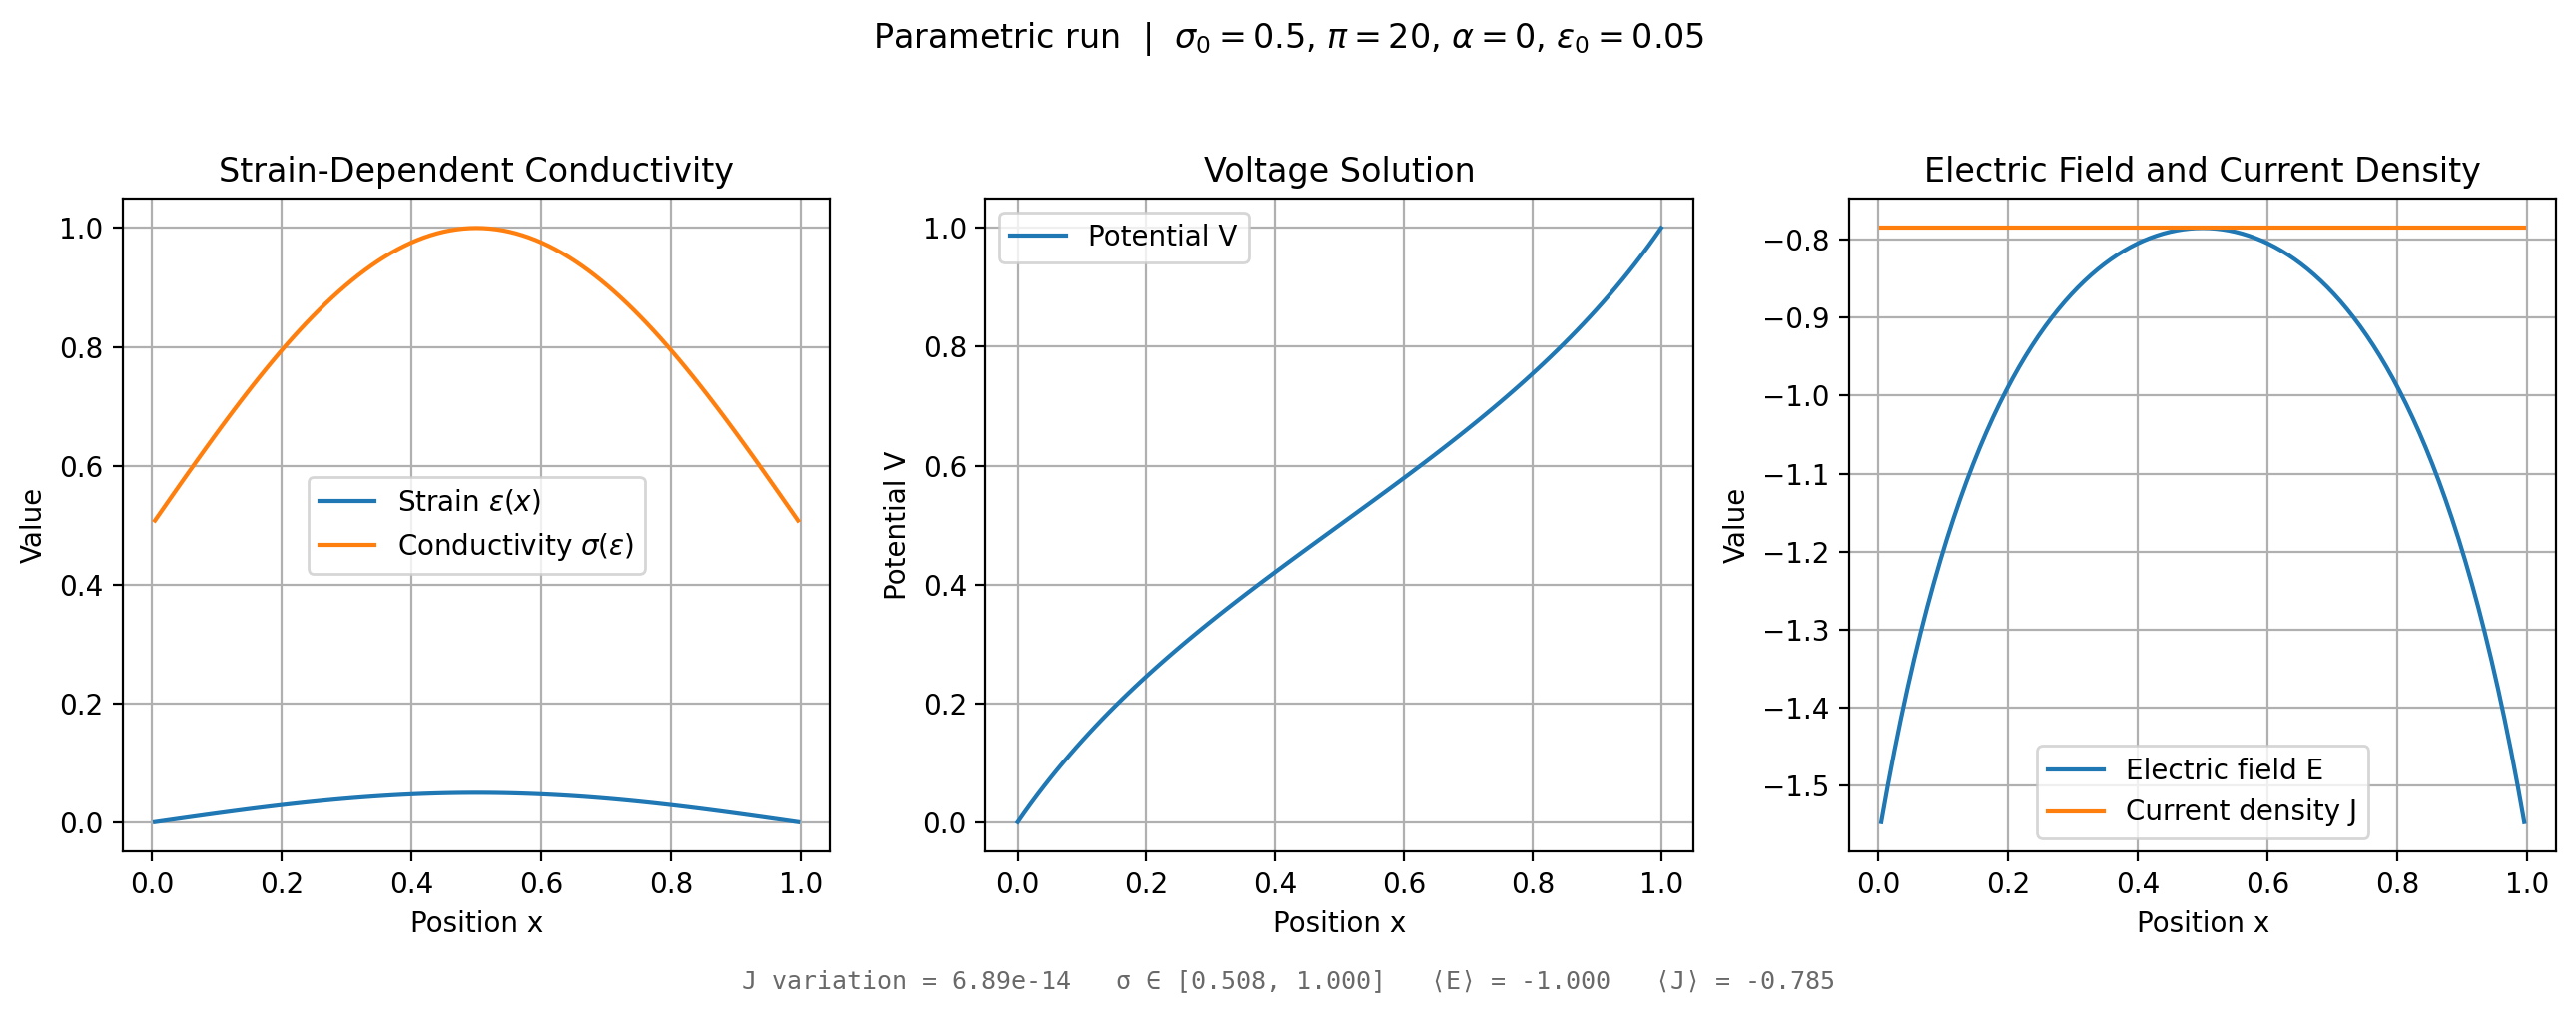
\includegraphics[width=0.75\textwidth]{Images/par_s0=0.5_pi=p20_a=p0_e0=0.05.png}
    %\fbox{\parbox[c][4cm][c]{0.75\linewidth}{\centering\textit{Placeholder: 
    %$\sigma(\varepsilon)$ vs.\ $\varepsilon$ for varying $\pi$ and $\alpha$.}}}
    \caption{Normalized conductivity $\sigma(\varepsilon)/\sigma_0$ as a function
    of strain $\varepsilon$ for representative values of the linear coefficient
    $\pi$ and the nonlinear coefficient $\alpha$. For small $|\varepsilon|$ the
    response is dominated by the linear term; the quadratic contribution becomes
    visible at larger strain amplitudes.}
    \label{fig:sigma_vs_eps}
\end{figure}



Physically, mechanical strain modifies the crystal lattice, which in turn alters
the electronic band structure, the carrier effective masses, and the dominant
scattering mechanisms. Within the Drude picture, the conductivity reads
\begin{equation}
    \sigma = \frac{n\,e^{2}\,\tau}{m^{*}},
    \label{eq:drude}
\end{equation}
where $n$ is the carrier density, $e$ the elementary charge, $\tau$ the momentum
relaxation time, and $m^{*}$ the effective mass. Strain therefore enters
$\sigma$ through all three microscopic quantities $n$, $\tau$, and $m^{*}$
simultaneously. Consequently, the Taylor expansion~\eqref{eq:taylor_normalized}
should be understood as an effective continuum-level description that subsumes
these microscopic contributions into the macroscopic coefficients $\pi$ and
$\alpha$, without requiring an explicit microscopic derivation.

\begin{figure}[ht]
    \centering
    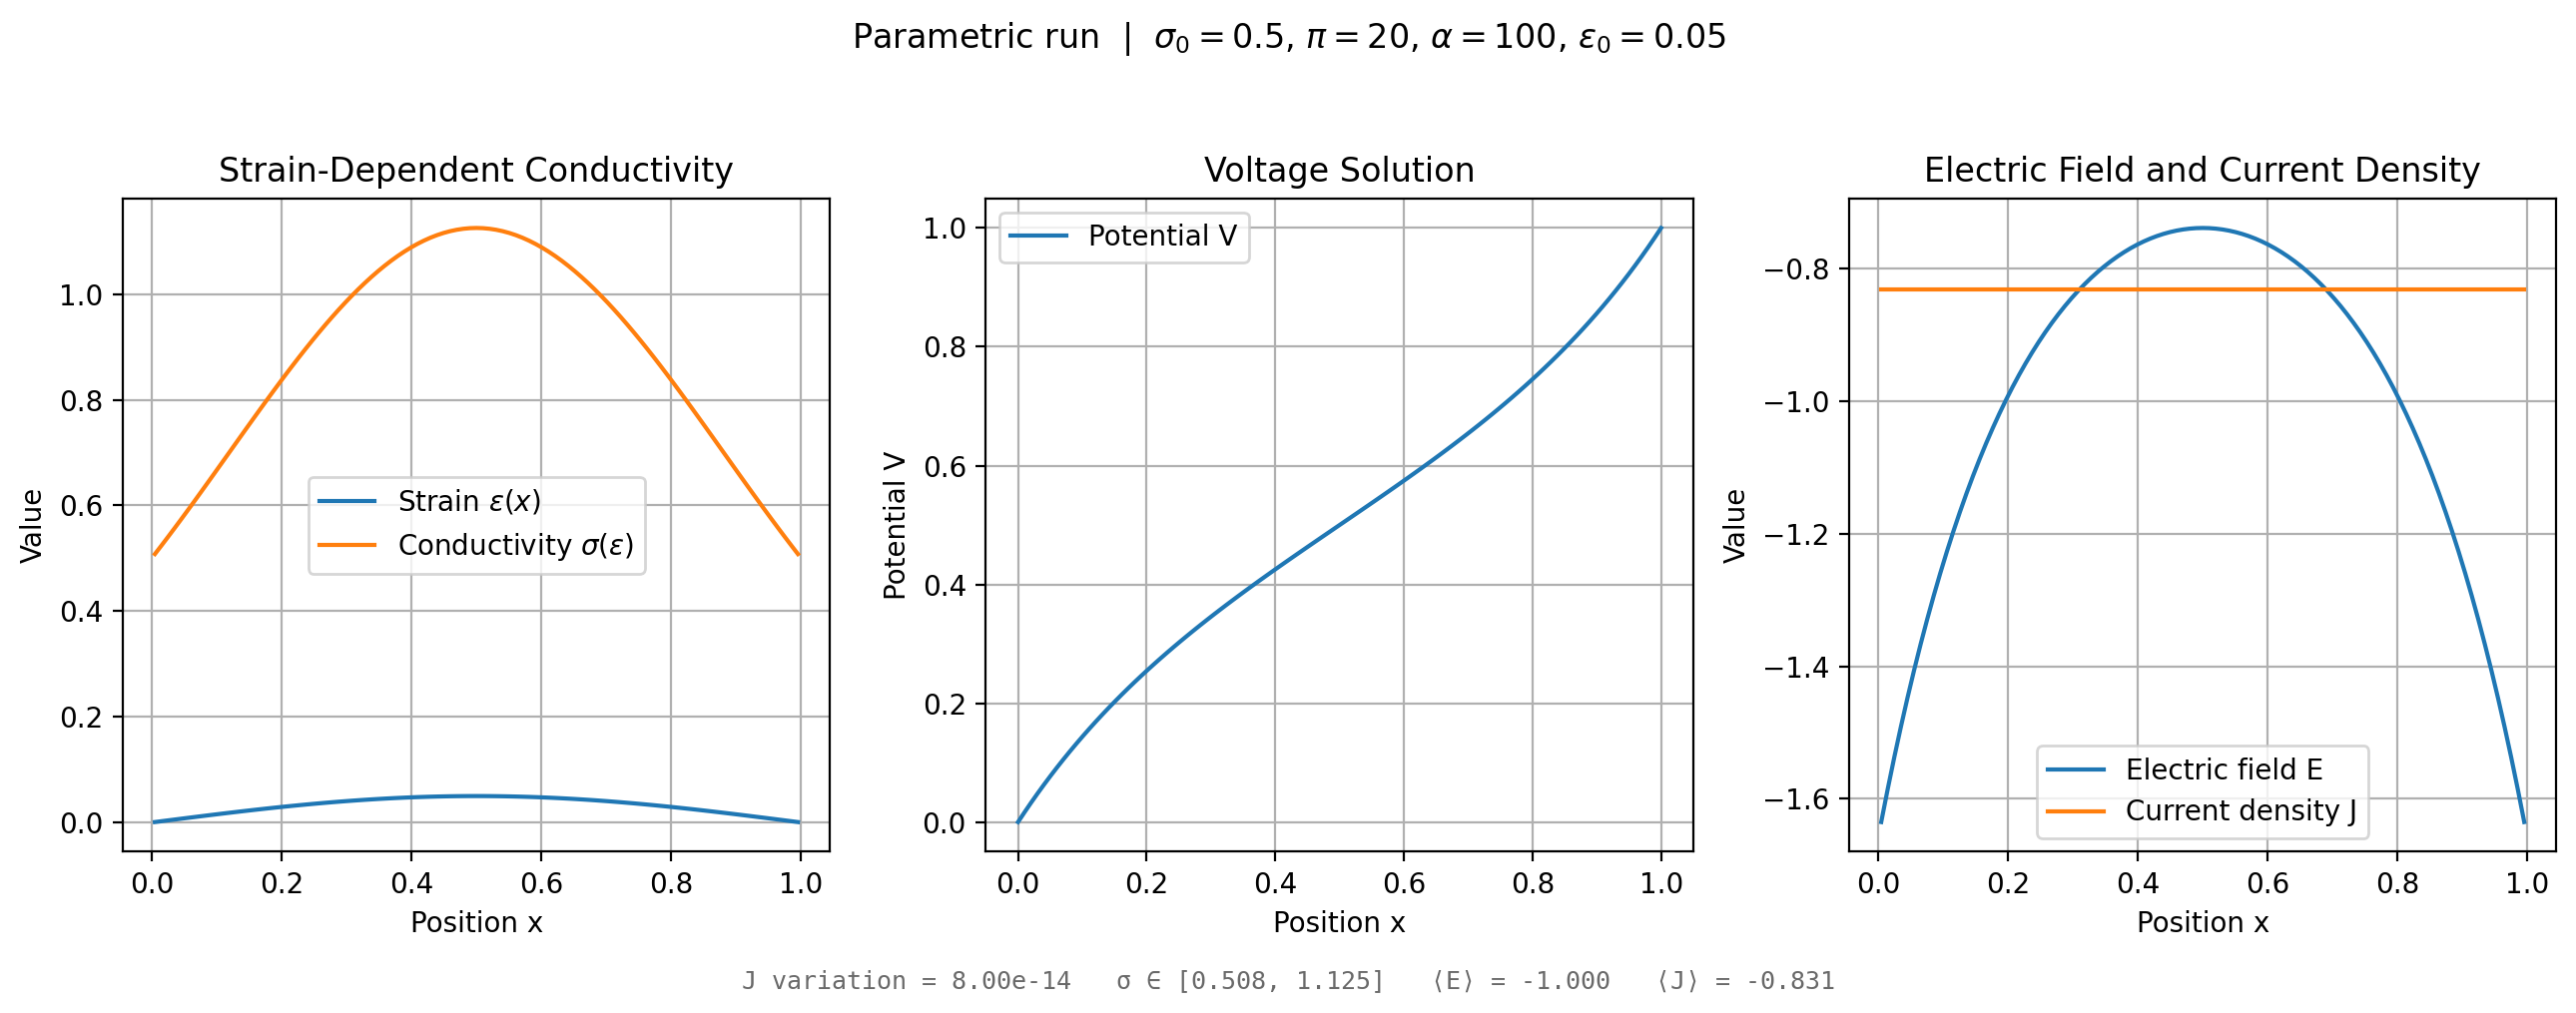
\includegraphics[width=0.75\textwidth]{Images/par_s0=0.5_pi=p20_a=p100_e0=0.05.png}
    %\fbox{\parbox[c][5cm][c]{0.85\linewidth}{\centering\textit{Placeholder:
    %Potential $V(x)$, electric field $E(x)$, and current density $J(x)$ for the
    %parametric study.}}}
    \caption{Finite element results for the one-dimensional coupled problem with
    strain-dependent conductivity~\eqref{eq:taylor_normalized}. A prescribed
    strain field $\varepsilon(x) = \varepsilon_0 \sin(\pi x)$ is used to
    illustrate the effect of the coefficients $\pi$ and $\alpha$ on the
    potential, electric field, and current density. The current density remains
    constant up to machine precision, confirming current conservation.}
    \label{fig:parametric_study}
\end{figure}

The parametric study based on~\eqref{eq:taylor_normalized} reveals a clear
separation between uncoupled and coupled regimes. For $\pi = \alpha = 0$ the
conductivity reduces to the constant baseline $\sigma = \sigma_0$, recovering a
linear potential profile $V(x)$, a constant electric field, and a uniform
current density; strain is present but does not influence transport. A non-zero
linear coefficient $\pi$ activates first-order piezoresistive coupling: the
conductivity now responds directly to the strain field, the electric field
redistributes accordingly, and the potential profile becomes nonlinear, while
the current density remains spatially constant in accordance with charge
conservation,
\begin{equation}
    \frac{dJ}{dx} = 0.
    \label{eq:current_cons}
\end{equation}
The sign and magnitude of $\pi$ control whether the conductivity locally
increases or decreases under deformation, and thereby the sensitivity of the
electrical response. The quadratic term $\alpha\varepsilon^{2}$ introduces
additional curvature in $\sigma(\varepsilon)$ and is typically subdominant for
small strains, but becomes appreciable at larger amplitudes. In all cases the
admissibility condition $\sigma(\varepsilon) > 0$ must be respected to preserve
physical meaning.

Across the tested configurations, the numerical results confirm that the current
density is conserved to machine precision, validating the finite element
implementation. The simulations show that the system maintains equilibrium by
compensating local variations in conductivity with corresponding adjustments in
the electric field, consistent with the constitutive relation $J = \sigma E$.
Representative parameter ranges for stable exploration are
$\sigma_0 \in [0.1, 2.0]$, $\pi \in [5, 20]$, $\alpha \in [0, 100]$, and strain
amplitudes $\varepsilon_0 \in [10^{-3}, 10^{-2}]$. Within this regime, the model
captures both linear and nonlinear piezoresistive behavior while remaining
numerically robust and physically interpretable.

% =====================================================================
%  Section 8 (MERGED): Physics-Informed Conductivity from First Principles
%
%  Replaces the existing Section 8 ("Toward a Physics-Informed Conductivity
%  Model") AND the standalone "Ab Initio Deformation Potentials" draft.
%
%  Requires in preamble: amsmath, amssymb, graphicx, booktabs
%  (optional: siunitx, hyperref). If you do NOT use siunitx, replace every
%  \SI{x}{unit} with "x unit" and \si{...} accordingly.
%
%  Figures: drop your images at the Images/ paths marked below.
%  Citations: \cite{hamaguchi} = your current ref [3]; add yu_cardona,
%  herring_vogt, pollak_cardona for the literature comparison (bibtex provided
%  separately).
%
%  Search "% ADJUST" for choices to confirm:
%    - PBE equilibrium gap value (0.62 eV used)
%    - tense/voice (written as completed work)
%    - cross-reference labels to other sections
% =====================================================================


\section{Physics-Informed Conductivity from First Principles}
\label{sec:physics-informed}

The parametric study of Section~\ref{sec:parametric}% ADJUST: label of "Parametric Solution"
treated the coefficients $\pi$ and $\alpha$ in
\begin{equation}
  \sigma(\varepsilon) = \sigma_0\big(1 + \pi\,\varepsilon + \alpha\,\varepsilon^2 + \dots\big)
  \label{eq:sigma-taylor}
\end{equation}
as free phenomenological parameters. This section removes that freedom in two
steps. First, deformation-potential theory fixes the \emph{form} of
$\sigma(\varepsilon)$ and expresses $\pi,\alpha$ in terms of a single material
coupling, the hydrostatic deformation potential $(a_c+a_v)$. Second, that
coupling---together with the shear deformation potentials---is computed directly
from density-functional theory (DFT), so the constitutive law is fixed entirely
from first principles rather than fitted. The overall pipeline is
\begin{equation}
  \varepsilon \;\longrightarrow\; H_s \;\longrightarrow\; \Delta E_g(\varepsilon)
  \;\longrightarrow\; n(\varepsilon) \;\longrightarrow\; \sigma(\varepsilon)
  \;\longrightarrow\; \nabla\!\cdot\!\big(\sigma\nabla V\big)=0 ,
  \label{eq:pipeline}
\end{equation}
with each arrow developed below, following the treatment in Hamaguchi
\cite{hamaguchi}.
\subsection{Strain Hamiltonian and band-gap shift}
\label{subsec:strain-hamiltonian}

When a crystal is uniformly strained, the periodic potential seen by the
electrons changes, perturbing the Bloch Hamiltonian. To first order in strain
this perturbation is called the strain Hamiltonian $H_s$; it couples the
electronic degrees of freedom linearly to the strain tensor $\varepsilon_{ij}$
through the deformation-potential operator $D_{ij}$ \cite{hamaguchi}:
\begin{equation}
  H = H_0 + H_s, \qquad H_s = \sum_{i,j} D_{ij}\,\varepsilon_{ij}.
  \label{eq:Hs}
\end{equation}
Here $H_0$ is the unstrained Bloch Hamiltonian and $D_{ij}$ encodes how each
strain component modifies the crystal potential; its explicit form involves
derivatives of the ionic pseudopotential but need not be evaluated
directly---only its band-state matrix elements appear in what follows.
To first order, the shift of a non-degenerate band edge $|n\rangle$ follows
from perturbation theory,
\begin{equation}
  \Delta E_n = \langle n|H_s|n\rangle
             = \sum_{i,j}\langle n|D_{ij}|n\rangle\,\varepsilon_{ij}.
  \label{eq:dEn}
\end{equation}
Separating the strain into a hydrostatic part,
\begin{equation}
  \varepsilon_h = \varepsilon_{xx}+\varepsilon_{yy}+\varepsilon_{zz} = \operatorname{Tr}\varepsilon,
  \label{eq:eps-h}
\end{equation}
and traceless shear components, the hydrostatic part shifts the band edges
rigidly while the shear part lifts degeneracies. The shear-induced splitting,
parameterized by the deformation potentials $b$ (equivalently the uniaxial
potential $\Xi_u$) and $d$ in the Picus--Bir framework, is anisotropic and
underlies the dominant piezoresistive response of doped silicon; it is
quantified in Section~\ref{subsec:dft-results} and its route into transport is
discussed in Section~\ref{subsec:outlook}. The hydrostatic shift of the gap is
\begin{equation}
  \Delta E_g(\varepsilon_h) \approx (a_c+a_v)\,\varepsilon_h,
  \label{eq:gap-shift}
\end{equation}
where $a_c$ and $a_v$ are the hydrostatic deformation potentials of the
conduction and valence band edges \cite{hamaguchi}.

\subsection{From band shift to carrier density}
\label{subsec:carrier-density}

In the non-degenerate Maxwell--Boltzmann limit the conduction-band electron
concentration is
\begin{equation}
  n = N_c \exp\!\left(-\frac{E_c - E_F}{k_B T}\right),
  \label{eq:n-extrinsic}
\end{equation}
and for an intrinsic semiconductor charge neutrality fixes the Fermi level near
mid-gap, giving
\begin{equation}
  n_i = \sqrt{N_c N_v}\,\exp\!\left(-\frac{E_g}{2 k_B T}\right),
  \label{eq:n-intrinsic}
\end{equation}
so that the strain-induced gap shift~\eqref{eq:gap-shift} produces a
multiplicative change in $n_i$, with the factor $1/2$ inherited from the
square root.

\subsection{Strain-dependent conductivity}
\label{subsec:sigma-law}

Combining the Drude form $\sigma = n e^2 \tau / m^\ast$ with the intrinsic
carrier density~\eqref{eq:n-intrinsic} and the linear gap
shift~\eqref{eq:gap-shift}, and assuming the mobility prefactor $\tau/m^\ast$
varies weakly with strain,
\begin{equation}
  \sigma(\varepsilon) \approx
  \sigma_0 \exp\!\left(-\frac{\Delta E_g(\varepsilon)}{2 k_B T}\right)
  = \sigma_0 \exp\!\left(-\frac{(a_c+a_v)\,\varepsilon_h}{2 k_B T}\right),
  \label{eq:sigma-exp}
\end{equation}
where $\sigma_0$ absorbs the unstrained prefactors. Introducing the
dimensionless coupling
\begin{equation}
  \kappa \equiv \frac{a_c+a_v}{2 k_B T},
  \label{eq:kappa}
\end{equation}
expanding the exponential for $|\kappa\varepsilon_h|\ll 1$, and matching
term by term with~\eqref{eq:sigma-taylor} gives
\begin{equation}
  \pi = -\kappa = -\frac{a_c+a_v}{2 k_B T}, \qquad
  \alpha = \tfrac{1}{2}\kappa^2 = \tfrac{1}{2}\!\left(\frac{a_c+a_v}{2 k_B T}\right)^{\!2}.
  \label{eq:pi-alpha}
\end{equation}
Equation~\eqref{eq:pi-alpha} is the key link: the phenomenological coefficients
acquire a microscopic meaning, their sign and relative magnitude fixed by a
single material parameter. For typical semiconductors with $(a_c+a_v)>0$, the
linear coefficient $\pi$ is negative---tensile hydrostatic strain widens the gap
and lowers the intrinsic conductivity---and $\alpha = \tfrac12\pi^2$, so the two
coefficients are not independent.

\subsection{Sensitivity to the coupling strength}
\label{subsec:sensitivity}

Before fixing $(a_c+a_v)$ from DFT, it is useful to map how the response depends
on it. Table~\ref{tab:coupling-sweep} evaluates~\eqref{eq:pi-alpha} at
$T=\SI{300}{K}$ ($k_B T = \SI{0.0259}{eV}$) for three representative couplings.
Even a modest coupling of \SI{1}{eV} gives $|\pi|\approx19$, at the upper end of
the phenomenological range $\pi\in[5,20]$ used in Section~\ref{sec:parametric};
the first-principles value obtained below
(Section~\ref{subsec:firstprinciples-pi}) falls between the moderate and strong
cases.

\begin{table}[ht]
  \centering
  \begin{tabular}{lcccc}
    \toprule
    case & $a_c+a_v$ [eV] & $\varepsilon_0$ & $\pi$ & $\alpha$ \\
    \midrule
    weak     & 0.3 & $5\times10^{-3}$ & $-5.80$  & $1.68\times10^{1}$ \\
    moderate & 1.0 & $5\times10^{-3}$ & $-19.34$ & $1.87\times10^{2}$ \\
    strong   & 3.0 & $3\times10^{-3}$ & $-58.02$ & $1.68\times10^{3}$ \\
    \midrule
    \textbf{this work (DFT)} & \textbf{1.83} & $\le10^{-2}$ & $\mathbf{-35.4}$ & $\mathbf{6.3\times10^{2}}$ \\
    \bottomrule
  \end{tabular}
  \caption{Coefficients $\pi$ and $\alpha$ from~\eqref{eq:pi-alpha} at
  $T=\SI{300}{K}$. The first three rows are a sensitivity sweep over
  representative couplings; the last row uses the first-principles value
  $a_c+a_v=\SI{1.83}{eV}$ determined in Section~\ref{subsec:dft-results}.}
  \label{tab:coupling-sweep}
\end{table}

The exponential law~\eqref{eq:sigma-exp} and its Taylor
truncation~\eqref{eq:sigma-taylor} are compared in
Figure~\ref{fig:sigma-exp-taylor}. For weak and moderate coupling the two are
indistinguishable across $|\varepsilon|\le0.02$; for strong coupling the Taylor
form begins to miss the tensile/compressive asymmetry of the exponential.

\begin{figure}[ht]
  \centering
  %\includegraphics[width=0.8\linewidth]{Images/sigma_exp_taylor.png}
  \caption{Normalized conductivity $\sigma(\varepsilon)/\sigma_0$ versus strain
  for three couplings at $T=\SI{300}{K}$. Solid: exponential
  law~\eqref{eq:sigma-exp}; dashed: Taylor approximation~\eqref{eq:sigma-taylor}
  with the coefficients~\eqref{eq:pi-alpha}.}
  \label{fig:sigma-exp-taylor}
\end{figure}

\subsection{Coupled finite-element solution}
\label{subsec:coupled-fem}

The one-dimensional conductivity equation~\eqref{eq:1d-cond}% ADJUST: label of div(sigma grad V)=0
is solved with the physics-informed law~\eqref{eq:sigma-exp} for a prescribed
strain profile $\varepsilon(x)=\varepsilon_0\sin(\pi x)$ on $[0,1]$ with
$V(0)=0,\,V(1)=1$. The mechanical assembly, linear solve, and post-processing
are unchanged from Section~\ref{sec:parametric}; only the local material law is
replaced.

Figure~\ref{fig:fem-coupled} shows the moderate case
($a_c+a_v=\SI{1}{eV}$, $\varepsilon_0=5\times10^{-3}$): the strain modulates the
conductivity, the potential bows away from the linear baseline, the electric
field develops a compensating spatial variation, and the current density remains
constant to machine precision---the discrete statement of $\nabla\!\cdot\!J=0$
and the principal consistency check. The exponential and Taylor laws are
numerically indistinguishable at this amplitude, consistent
with~\eqref{eq:pi-alpha}. Figure~\ref{fig:fem-sweep} shows that the departure of
$V(x)$ and $E(x)$ from the uncoupled baseline grows with $(a_c+a_v)$.

\begin{figure}[ht]
  \centering
  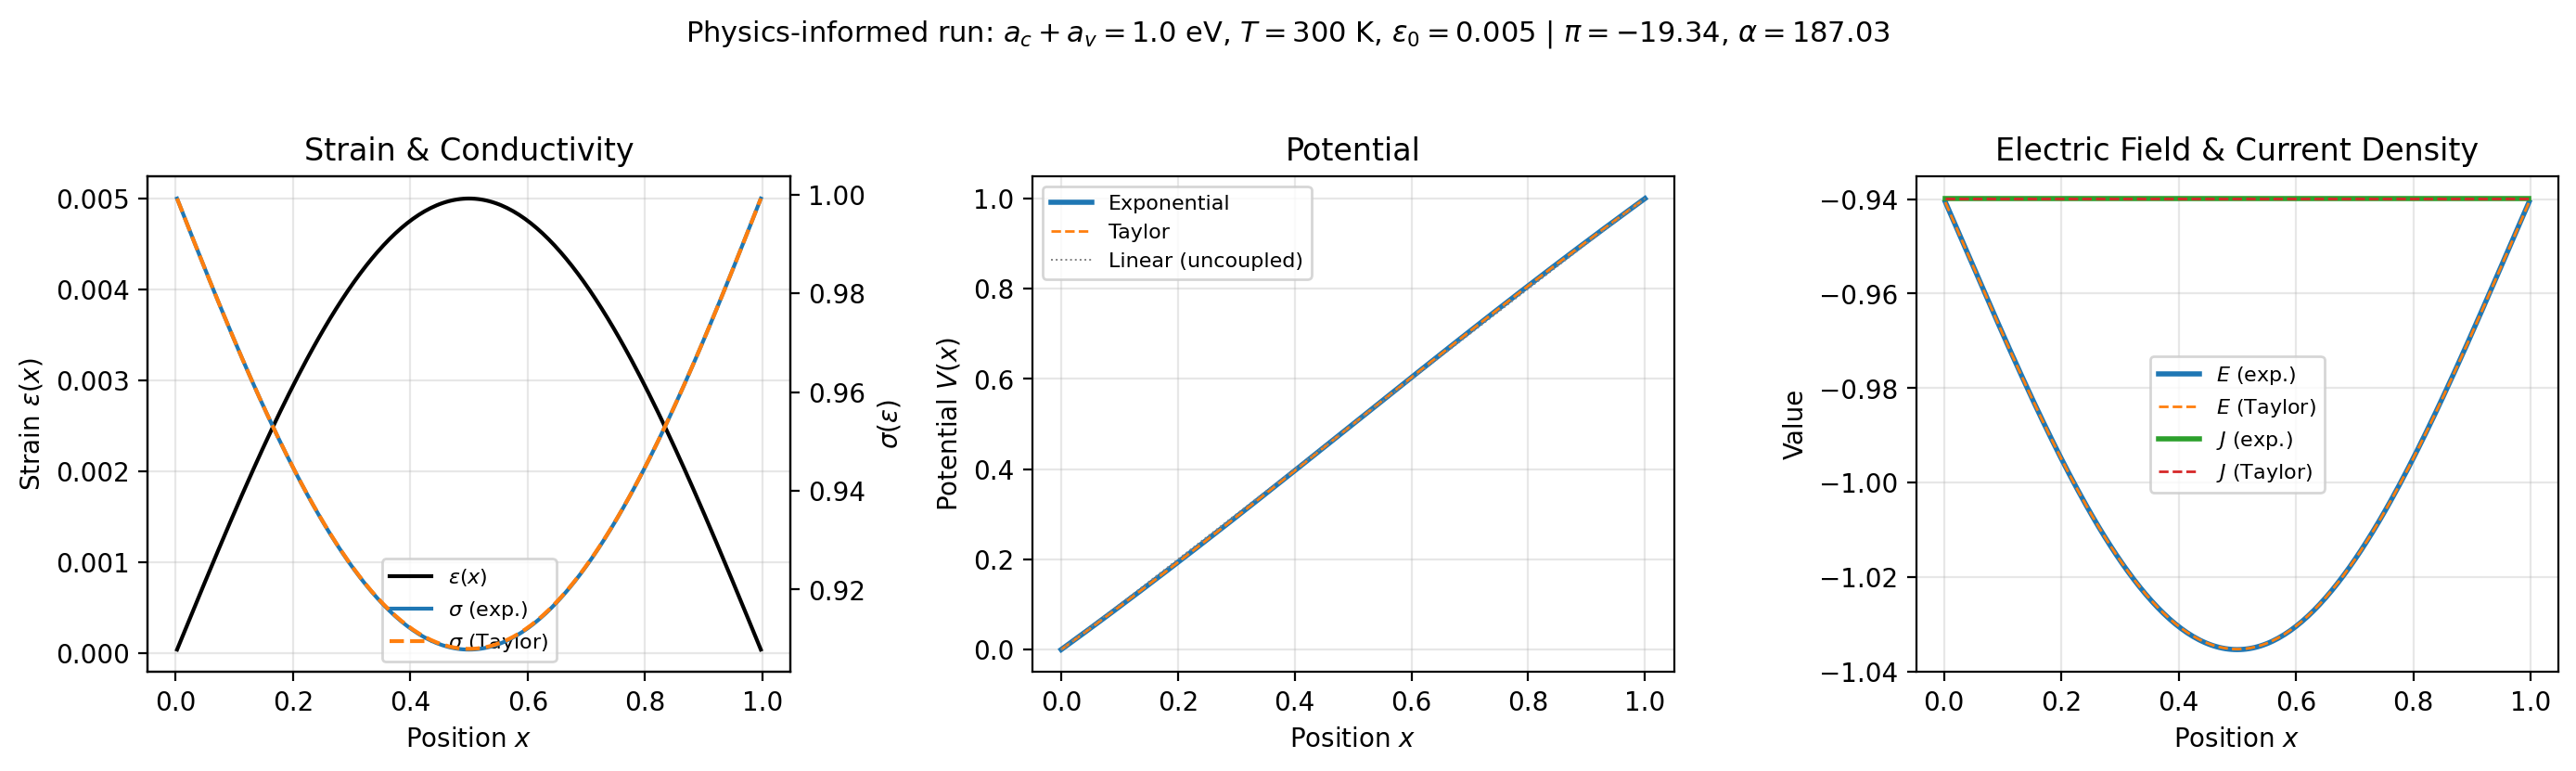
\includegraphics[width=0.95\linewidth]{Images/fig_FEM_moderate.png}
  \caption{Finite-element solution of the coupled problem with the
  physics-informed law~\eqref{eq:sigma-exp} for $a_c+a_v=\SI{1}{eV}$ at
  $T=\SI{300}{K}$, $\varepsilon_0=5\times10^{-3}$. Left: strain and conductivity;
  middle: potential; right: electric field and current density. $J$ is constant
  to machine precision while $E$ varies to compensate $\sigma(x)$.}
  \label{fig:fem-coupled}
\end{figure}

\begin{figure}[ht]
  \centering
  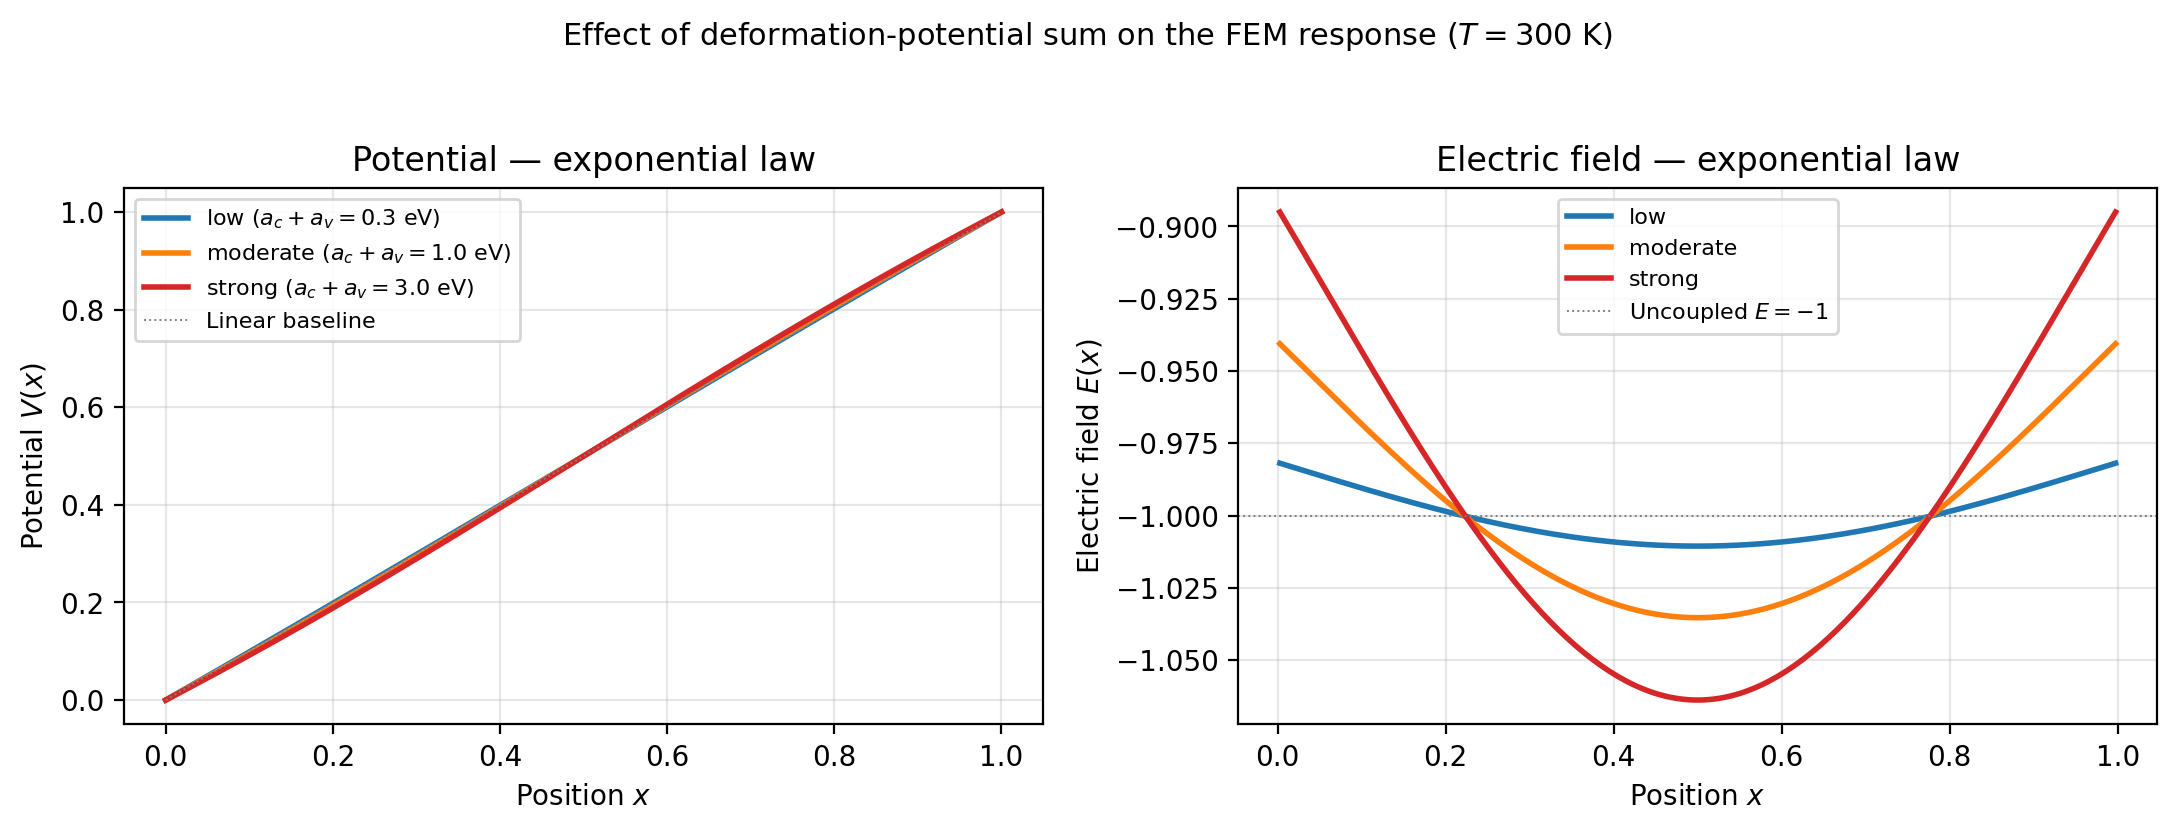
\includegraphics[width=0.95\linewidth]{Images/fig_compare_cases.png}
  \caption{Effect of the deformation-potential sum on the FEM response at
  $T=\SI{300}{K}$. Left: potential profiles for the three cases of
  Table~\ref{tab:coupling-sweep}; right: electric field. The deviation from the
  uncoupled value $E=-1$ grows with the coupling strength.}
  \label{fig:fem-sweep}
\end{figure}

% =====================================================================
%  DETERMINATION HALF — first-principles DFT
% =====================================================================

\subsection{First-principles deformation potentials}
\label{subsec:dft-results}
The coupling $(a_c+a_v)$ used above is only one of three independent deformation
potentials of cubic silicon. The other two---the uniaxial potential $\Xi_u$ and
the shear potential $d$---do not enter the scalar law~\eqref{eq:sigma-exp}, but
they govern the dominant, anisotropic part of silicon's piezoresistance through
valley repopulation and valence-band splitting (Section~\ref{subsec:outlook}).
All three are computed here from the band structure: the hydrostatic potential to
fix the constitutive law, and the shear potentials to supply the inputs the full
transport treatment requires. The physical chain is exactly the
pipeline~\eqref{eq:pipeline}: applied strain moves the atoms, which changes the
potential the electrons feel, which shifts and splits the bands; the slopes of
those shifts with respect to strain are the deformation potentials. Cubic symmetry
fixes how many are independent and which strain isolates each one.

\paragraph{One strain mode per deformation potential.}
A general strain of silicon separates into three symmetry-distinct modes, each
isolating one deformation potential (Table~\ref{tab:strain-modes}). This is what
makes the calculation efficient: three symmetry-pure strains suffice, rather
than a scan over arbitrary deformations.

\begin{table}[ht]
  \centering
  \begin{tabular}{lll}
    \toprule
    Strain mode & Effect on the bands & Probes \\
    \midrule
    Hydrostatic (volume) & gap shifts, no splitting          & $a = a_c+a_v$ \\
    Tetragonal (one axis) & $\langle100\rangle$ valleys split & $\Xi_u$ \\
    Trigonal shear (angles) & valence top at $\Gamma$ splits  & $d$ \\
    \bottomrule
  \end{tabular}
  \caption{The three symmetry-pure strain modes and the deformation potential
  each isolates. Hydrostatic strain keeps all directions equivalent (no
  splitting); the tetragonal and shear modes break symmetry and lift specific
  degeneracies.}
  \label{tab:strain-modes}
\end{table}

\paragraph{Computational method.}
Calculations use VASP with PAW PBE potentials, a plane-wave cutoff of
\SI{320}{eV}, and the relaxed primitive cell of silicon as the
$\varepsilon=0$ reference. Crystal symmetry is disabled (\texttt{ISYM}=0) so that
a small symmetry-lowering strain is not folded back to the cubic structure,
which would erase the splitting being measured. Each strained structure is run
in stages: a self-consistent calculation on a uniform $\mathbf k$-mesh converges
the charge density, then a non-self-consistent calculation produces the bands
along a high-symmetry path. For the trigonal-shear runs an ionic relaxation at
fixed cell shape precedes these steps, because the two atoms of the diamond
basis displace relative to one another under shear (the internal-strain or
Kleinman effect); the hydrostatic and tetragonal modes need no such relaxation.
Strain amplitudes of $\pm0.2,0.5,1.0\,\%$ are applied, and each deformation
potential is obtained as the slope of a band feature versus strain. The
equilibrium PBE band structure is shown in Figure~\ref{fig:bands-eq}; PBE
underestimates the absolute gap ($E_g(0)\approx\SI{0.62}{eV}$% ADJUST: PBE gap value
versus the experimental \SI{1.12}{eV}), but the deformation potentials are
\emph{slopes} and are far less sensitive to this error than the absolute gap. 
\begin{RL}
However one can use corrections for example in \cite{DFT_Correction}.
\end{RL}

\begin{figure}[ht]
  \centering
  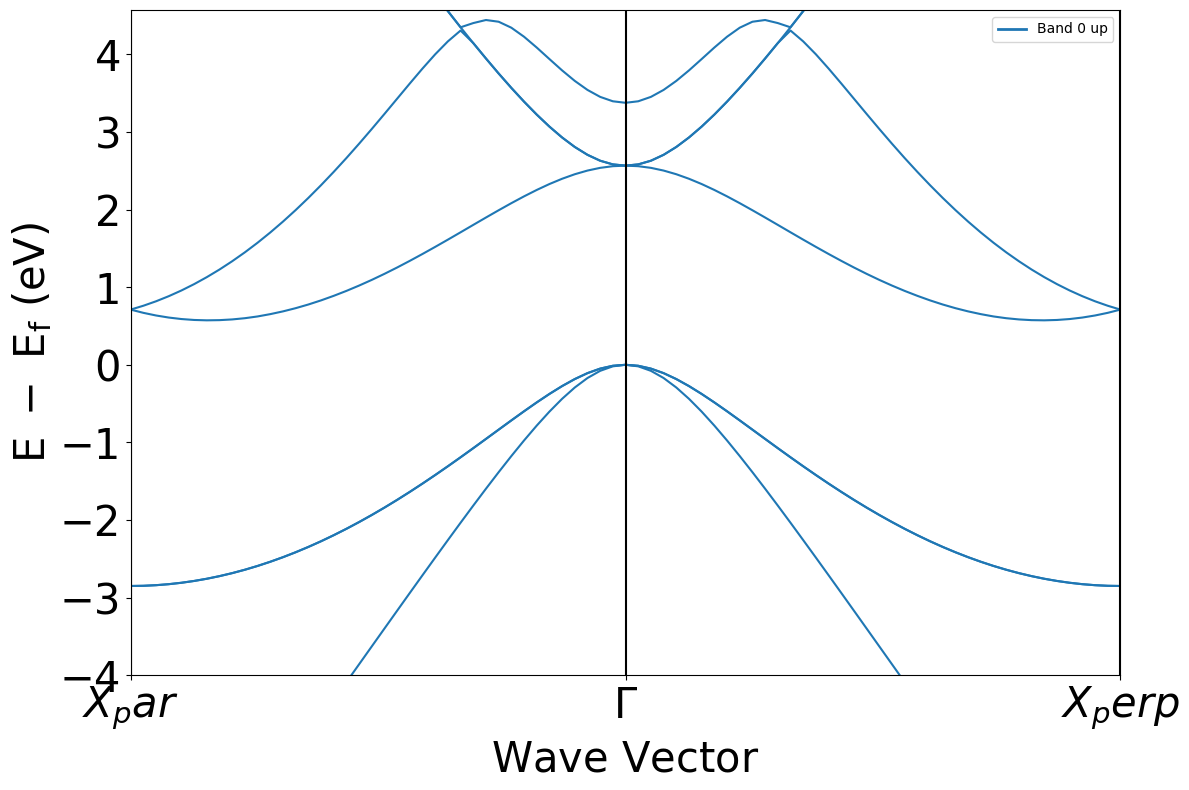
\includegraphics[width=0.75\linewidth]{Images/bands_equilibrium.png}
  \caption{Equilibrium band structure of silicon (VASP, PBE) along the
  dual-X path $X_\parallel$--$\Gamma$--$X_\perp$, energies referenced to the
  valence-band maximum. At zero strain the two X points are degenerate; the
  valence maximum sits at $\Gamma$ and the conduction minima near $X$,
  reproducing the indirect gap.}
  \label{fig:bands-eq}
\end{figure}

\paragraph{Extraction and results.}
The extraction relations follow from the band features in
Table~\ref{tab:strain-modes}:
\begin{align}
  a = a_c+a_v &= \frac{\mathrm{d}E_g}{\mathrm{d}\,\operatorname{Tr}\varepsilon}, \\[2pt]
  \Xi_u &= \frac{\mathrm{d}}{\mathrm{d}\varepsilon}\big[E_c(X_\parallel)-E_c(X_\perp)\big], \\[2pt]
  |d| &= \frac{\Delta E_{\Gamma_{25'}}}{3\sqrt{3}\,\varepsilon_{xy}} .
\end{align}
The band structures for the three modes at $\varepsilon=-1\%,0,+1\%$ are shown
in Figure~\ref{fig:bands-modes}, and the linear fits behind each potential in
Figure~\ref{fig:dp-extraction}. The resulting values are collected in
Table~\ref{tab:dp-values}.

\begin{figure}[ht]
  \centering
  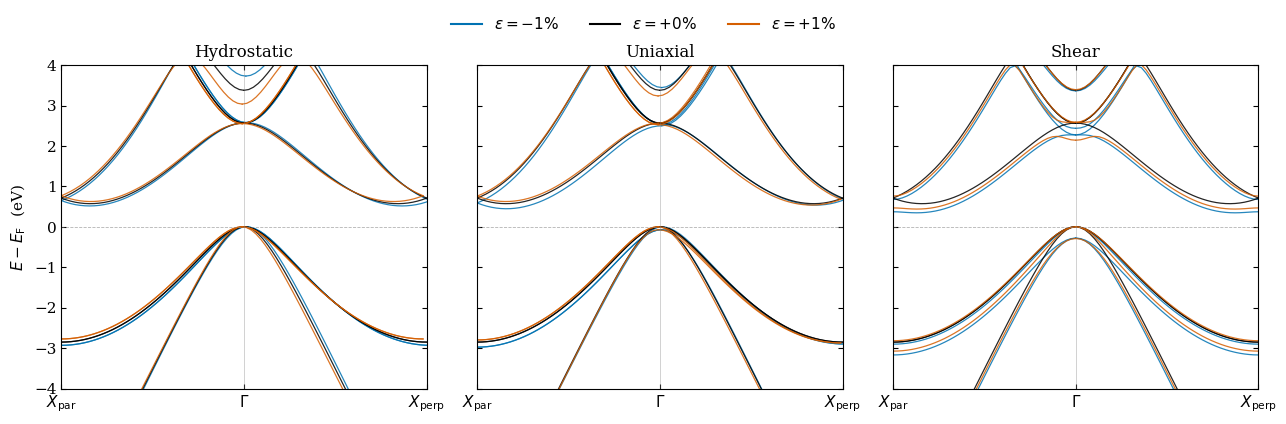
\includegraphics[width=0.95\linewidth]{Images/bands_strain_modes.png}
  \caption{Band structure of silicon at $\varepsilon=-1\%,0,+1\%$ for the three
  strain modes. Hydrostatic strain shifts the gap with no splitting; tetragonal
  strain splits the conduction valleys ($X_\parallel$ vs.\ $X_\perp$); trigonal
  shear splits the valence-band maximum at $\Gamma$.}
  \label{fig:bands-modes}
\end{figure}

\begin{figure}[ht]
  \centering
  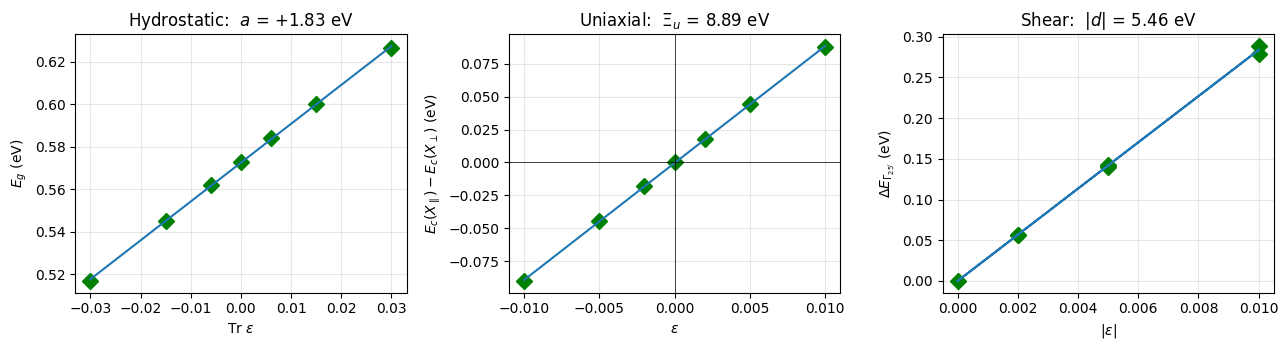
\includegraphics[width=0.95\linewidth]{Images/dp_extraction.png}
  \caption{Deformation potentials as slopes: gap versus hydrostatic strain
  ($a$); valley splitting versus tetragonal strain ($\Xi_u$), passing through
  zero at $\varepsilon=0$; valence splitting versus shear magnitude ($|d|$). The
  slopes give the values of Table~\ref{tab:dp-values}.}
  \label{fig:dp-extraction}
\end{figure}

\begin{table}[ht]
  \centering
  \begin{tabular}{llll}
    \toprule
    Deformation potential & This work & Literature (Si) & Source \\
    \midrule
    $a = a_c+a_v$            & $+1.83$ eV       & $\sim +1.5$       & \cite{yu_cardona} \\
    $\Xi_u$                  & $+8.89$ eV       & $9.0 \pm 2$       & \cite{yu_cardona, herring_vogt} \\
    $|d|$                    & $5.46$ eV        & $\sim 5.3\;(d<0)$ & \cite{yu_cardona, pollak_cardona} \\
    $\mathrm{d}E_g/\mathrm{d}P=-a/B$ & $-18.7$ meV/GPa & $\sim -15$ & \cite{yu_cardona} \\
    \bottomrule
  \end{tabular}
  \caption{Deformation potentials of silicon from the three strain sweeps,
  compared with literature. The gap potential $a$ carries its sign because it
  sets the sign of $\pi$ via~\eqref{eq:pi-alpha}; $\Xi_u$ is a positive splitting
  coefficient; $d$ is reported as a magnitude, the standard convention being
  $d<0$. The pressure coefficient $\mathrm{d}E_g/\mathrm{d}P=-a/B$ (bulk modulus
  $B\approx\SI{98}{GPa}$) is a convention-independent comparison with experiment.}
  \label{tab:dp-values}
\end{table}

Each sweep reproduces the behaviour symmetry requires, which validates the
calculation independently of the fitted numbers. Hydrostatic strain shifts the
gap monotonically with no splitting; tetragonal strain produces a valley
splitting that vanishes at $\varepsilon=0$ and reverses sign with the strain (the 
transverse valleys forming the conduction minimum under tension, the strain-axis valleys under compression); trigonal
shear splits the $\Gamma_{25'}$ valence triplet symmetrically in $\pm\varepsilon$,
the signature of a pure traceless shear. The negative pressure coefficient,
close to the measured value, confirms the full chain from atomic structure to
band gap.
\subsection{First-principles \texorpdfstring{$\pi$}{pi}
            and \texorpdfstring{$\alpha$}{alpha}}
\label{subsec:firstprinciples-pi}

Inserting the computed $a=a_c+a_v=\SI{1.83}{eV}$ into~\eqref{eq:kappa}
and~\eqref{eq:pi-alpha} at $T=\SI{300}{K}$ gives
\begin{equation}
  \kappa = \frac{a_c+a_v}{2k_BT} = 35.4, \qquad
  \pi = -35.4, \qquad
  \alpha = \tfrac12\kappa^2 = 626.
  \label{eq:firstprinciples-pi}
\end{equation}
This is the last row of Table~\ref{tab:coupling-sweep}: silicon sits between the
moderate and strong cases, the coupling is sizeable, and the negative sign
confirms that tensile hydrostatic strain lowers the intrinsic conductivity. The
representative parameters of Section~\ref{sec:parametric} are thereby replaced by
a single computed value, and the hydrostatic part of $\sigma(\varepsilon)$
in~\eqref{eq:sigma-exp} is fixed entirely from first principles.
Figure~\ref{fig:fem-coupled2} shows the resulting finite-element solution;
the potential deviates visibly from the uncoupled baseline, confirming that
$a=\SI{1.83}{eV}$ produces a physically meaningful piezoresistive response.

\begin{figure}[ht]
  \centering
  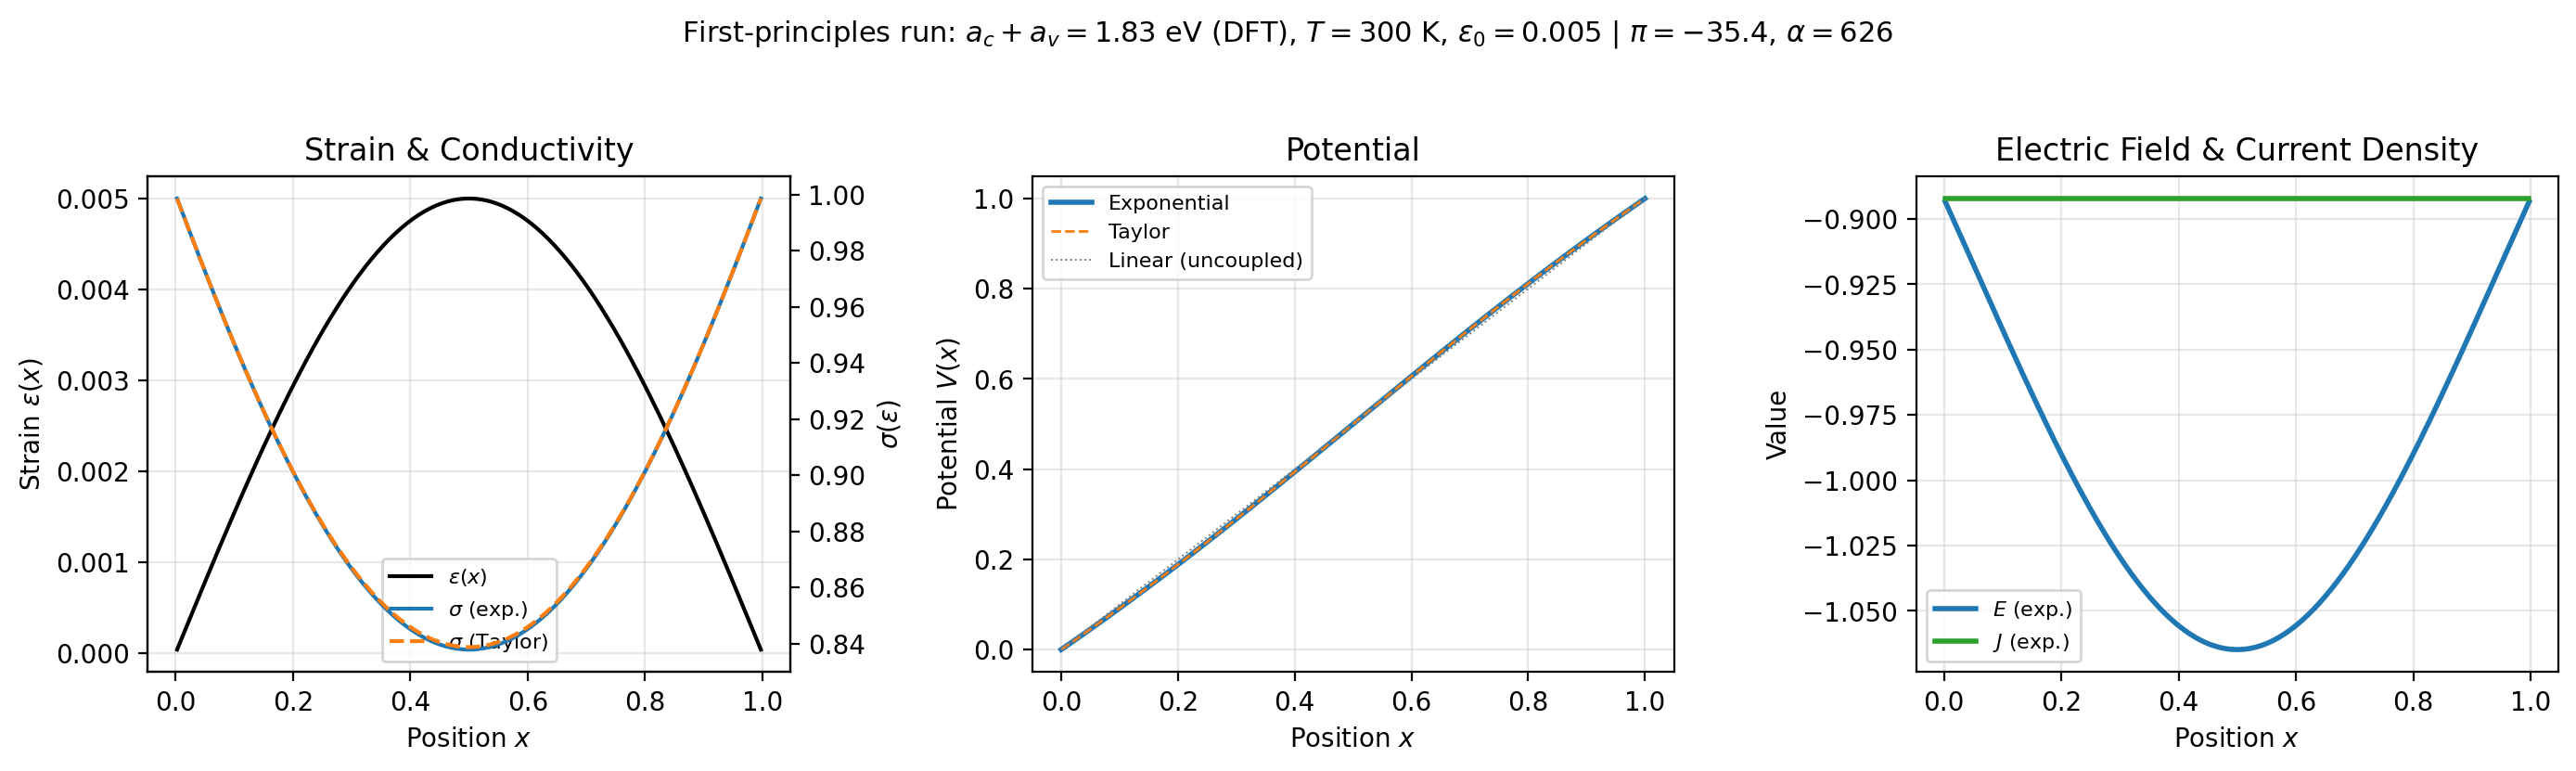
\includegraphics[width=0.95\linewidth]{Images/fem_dft.png}
  \caption{Finite-element solution with the physics-informed
  law~\eqref{eq:sigma-exp} for $a_c+a_v=\SI{1.83}{eV}$ (DFT, $\pi=-35.4$,
  $\alpha=626$) at $T=\SI{300}{K}$, $\varepsilon_0=5\times10^{-3}$. Left: strain
  and conductivity; middle: potential; right: electric field and current density.
  $J$ is constant to machine precision while $E$ compensates $\sigma(x)$,
  completing the first-principles pipeline~\eqref{eq:pipeline}.}
  \label{fig:fem-coupled2}
\end{figure}
\subsection{Outlook: the transport step and the role of shear strain}
\label{subsec:outlook}

The constitutive law developed above is complete and self-contained, but it
captures only one of the two channels through which strain alters conductivity,
and not the dominant one for the devices of interest.

\paragraph{Two channels, one implemented.}
Through $\sigma = n e \mu$, strain can act on the carrier density $n$ or on the
mobility $\mu$. The exponential law~\eqref{eq:sigma-exp} is the \emph{density}
channel: hydrostatic strain shifts the gap, the gap shifts $n$ through
Maxwell--Boltzmann statistics, and only the hydrostatic potential $a=a_c+a_v$
enters. This channel is isotropic by construction---it depends on $\varepsilon$
only through the scalar $\operatorname{Tr}\varepsilon$---and is sub-dominant in
doped silicon, where $n\approx N_D$ is pinned by the dopants and responds only
weakly to a gap shift.

\paragraph{Why the shear potentials were computed.}
The large, technologically exploited piezoresistance of silicon, first measured
by Smith \cite{smith1954}, comes from the \emph{mobility} channel and is anisotropic.
Uniaxial $\langle100\rangle$ strain splits the six conduction valleys (coefficient
$\Xi_u$); electrons repopulate toward the lowered valleys, changing the
direction-averaged conductivity mass and hence $\mu$. This is the origin of the
large $\pi_{11}$ of $n$-type silicon. Trigonal shear splits the valence-band
maximum (coefficient $d$), redistributing holes among bands of different
curvature, which dominates $\pi_{44}$ of $p$-type silicon. The potentials $\Xi_u$
and $d$ in Table~\ref{tab:dp-values} are therefore not auxiliary: they
parameterize the principal piezoresistive effect. They are absent from
$\sigma(\varepsilon)$ here only because the carrier-density argument has no place
for them---valley repopulation changes mobility, not carrier number.

\paragraph{Where the Boltzmann transport equation enters.}
Routing $\Xi_u$ and $d$ into transport requires the conductivity in its full
Boltzmann tensor form,
\begin{equation}
  \sigma_{ij} = \frac{e^2}{4\pi^3}\sum_n \int
  v^n_i(\mathbf k)\,v^n_j(\mathbf k)\,\tau_n(\mathbf k)
  \left(-\frac{\partial f_0}{\partial E}\right)\mathrm d\mathbf k ,
  \label{eq:bte-outlook}
\end{equation}
rather than the scalar $\sigma = ne\mu$. Strain enters~\eqref{eq:bte-outlook}
through the shifted band energies $\delta E_n = \Xi_{ij}\varepsilon_{ij}$, which
modify the group velocities $v^n_i=\hbar^{-1}\partial E_n/\partial k_i$, the
valley occupations through $-\partial f_0/\partial E$, and the intervalley
relaxation times $\tau_n$. The result is a genuine tensor
$\sigma_{ij}(\varepsilon)$ carrying the anisotropy that the scalar law cannot
represent. Equation~\eqref{eq:bte-outlook} requires two ingredients the present
work does not yet supply: the strained band structure on a dense $\mathbf k$-mesh,
available in principle from the same VASP runs used here, and the relaxation times
$\tau_n(\mathbf k)$, which demand a separate electron--phonon calculation
(density-functional perturbation theory coupled to a Boltzmann-transport solver).
The deformation potentials of Section~\ref{subsec:dft-results} are exactly the
band-structure inputs this step consumes; the relaxation times are the remaining
piece.

\paragraph{Further approximations.}
Two narrower assumptions accompany the density channel. The intrinsic carrier
density~\eqref{eq:n-intrinsic} overstates the gap contribution in doped devices,
where the mobility channel above dominates; and the Maxwell--Boltzmann
form~\eqref{eq:n-extrinsic} fails at high doping or low temperature, where
Fermi--Dirac statistics are required. Neither alters the structure of the
pipeline~\eqref{eq:pipeline} or the finite-element infrastructure of
Section~\ref{sec:parametric}: each refinement replaces the local material law
while leaving the assembly and solver untouched.



% =====================================================================
%  Uniaxial channel
% =====================================================================


\subsection{Uniaxial Channel: Valley Repopulation}
\label{subsec:uniaxial}

In hydrostatic channel we have developed through \ref{eq:Hs} (the trace part of 
strain tensor), the shift of bands calculations. We have also identified the anisotropic splitting
of the bands in traceless part of the tnesor. 

The route to transport for this part includes the electron mobility repopulation since the anisotropic
distribution of the valleys. This leads to study the redistribution of energy valleys, as an effect of 
applied uniaxial strain.


% [opening: contrast with hydrostatic — see rewrite below]

\paragraph{Symmetry of the six-valley splitting.} The uniaxial strain breaks the rotational symmetry(...). 
This leads to an anisotropic repopulation of the momenta along $<100>$, for Si and along $<111>$ for Ge /cite{hamaguchi}. 
%[the Herrin-Vogt term, the (100) grouping into 2+4, Table cross-ref]

\paragraph{Repopulation and the conductivity tensor.}
%[Boltzmann weights, cancellation of $a$, sigma = sum over six fixed M_i^{-1},
%the epsilon=0 isotropy gate as validation]

\paragraph{Extraction of $\pi_{11}-\pi_{12}$.}
%[strain-to-stress bridge, combined with the hydrostatic result to solve
%the 2x2 system, benchmark against Smith (1954)]

\paragraph{Role of the effective masses.}
%[m_l, m_t from DFT curvature at the valley minimum; note the classic
%cyclotron-resonance values this benchmarks against, \cite{hamaguchi} Eq. 2.26 —
%this is where your existing cyclotron-resonance sentence actually belongs,
%reframed as a validation check rather than a floating fact]

\input{Sections/DefPot.tex}

\section{Expected Outcome}

The expected outcome of this study is the development of a computational framework for analyzing strain-dependent electrical conduction 
in deformable materials. The framework combines continuum mechanics and electrical transport into a unified numerical model, 
enabling the systematic investigation of electromechanical coupling.

At the modeling level, the work provides a consistent formulation of conductivity as a strain-dependent quantity, 
together with a numerical implementation for solving the resulting coupled system. 
This allows for the analysis of how mechanical deformation influences electrical potential distribution, 
current density, and overall system sensitivity.

From a computational perspective, the study delivers a flexible pipeline that can accommodate different forms of the 
strain–conductivity relation, ranging from phenomenological descriptions to physically informed or data-driven models. 
This makes the framework adaptable to different materials and configurations.

Beyond the specific application, the results contribute to the understanding of nonlinear multiphysics systems 
involving coupling between deformation and transport phenomena. 
Potential applications include piezoresistive sensing, structural health monitoring, and functional materials design.

The developed framework also provides a foundation for future extensions toward multiscale modeling 
and more detailed transport descriptions.


\clearpage
\printbibliography

\end{document}
